\documentclass[ngerman,a4paper,order=firstname]{../../texmf/tex/latex/mathscript/mathscript}
\usepackage{../../texmf/tex/latex/mathoperators/mathoperators}

\title{\textbf{Lineare Algebra WS2017/18}}
\author{Dozent: Prof. Dr. Arno Fehm}

\begin{document}
\pagenumbering{roman}
\pagestyle{plain}

\maketitle

\hypertarget{tocpage}{}
\tableofcontents
\bookmark[dest=tocpage,level=1]{Inhaltsverzeichnis}

\pagebreak
\pagenumbering{arabic}
\pagestyle{fancy}

\chapter*{Vorwort}
Schön, dass du unser Skript für die Vorlesung \textit{Lineare Algebra und analytische Geometrie 1} bei Prof. Dr. Arno Fehm im WS2017/18 gefunden hast! \footnote{Obwohl man sagen kann, dass es in dieser Vorlesung nur um Lineare Algebra ging, der Teil mit der analytischen Geometrie wurde vernachlässigt. Liegt wahrscheinlich auch daran, dass es demnächst eine Reform der Studienordnung gibt, in der aus der Vorlesung \textit{Lineare Algebra und analytische Geometrie} die Vorlesung \textit{Einführung in die Lineare Algebra} wird.}

Wir verwalten dieses Skript mittels Github \footnote{Github ist eine Seite, mit der man Quelltext online verwalten kann. Dies ist dahingehend ganz nützlich, dass man die Quelltext-Dateien relativ einfach miteinander synchronisieren kann, wenn man mit mehren Leuten an einem Projekt arbeitet.}, d.h. du findest den gesamten \LaTeX-Quelltext auf \url{https://github.com/henrydatei/TUD_MATH_BA}. Unser Ziel ist, für alle Pflichtveranstaltungen von \textit{Mathematik-Bachelor} ein gut lesbares Skript anzubieten. Für die Programme, die in den Übungen zur Vorlesung \textit{Programmieren für Mathematiker} geschrieben werden sollen, habe ich ein eigenes Repository eingerichtet; es findet sich bei \url{https://github.com/henrydatei/TU_PROG}.

Du kannst dir gerne dort die \LaTeX-Quelldateien herunterladen, die Dateien für exakt dieses Skript sind im Ordner \texttt{1. Semester/LAAG ueberarbeitet}. Es lohnt sich auf jeden Fall während des Studiums die Skriptsprache \LaTeX{} zu lernen, denn Dokumente, die viele mathematische oder physikalische Formeln enthalten, lassen sich sehr gut mittels \LaTeX{} darstellen, in Word oder anderen Office-Programmen sieht so etwas dann eher dürftig aus.

\LaTeX{} zu lernen ist gar nicht so schwierig, ich habe dafür am Anfang des ersten Semesters wenige Wochen benötigt, dann kannte ich die wichtigsten Befehle und konnte den Vorgänger dieses Skriptes schreiben (\texttt{1. Semester/LAAG}, Vorsicht: hässlich, aber der Quelltext ist relativ gut verständlich).

Es sei an dieser Stelle darauf hingewiesen (wie in jedem anderem Skript auch \smiley{}), dass dieses Skript nicht den Besuch der Vorlesungen ersetzen kann. Es könnte sein, dass Prof. Fehm seine Vorlesung immer mal wieder an die Studenten anpasst; wahrscheinlich immer dann, wenn die Prüfungsergebnisse zu schlecht waren. Nichtsdestotrotz veröffentlicht Prof. Fehm sein Skript auf seiner Homepage \url{http://www.math.tu-dresden.de/~afehm/lehre.html}. Allerdings ist dieses Skript recht hässlich, besonders was die Übersichtlichkeit angeht.

Wir möchten deswegen ein Skript bereitstellen, dass zum einen übersichtlich ist, zum anderen \textit{alle} Inhalt aus der Vorlesung enthält, das sind insbesondere Diagramme, die sich nicht im offiziellen Skript befinden, aber das Verständnis des Inhalts deutlich erleichtern. Ich denke, dass uns dies erfolgreich gelungen ist.

Trotz intensivem Korrekturlesen können sich immer noch Fehler in diesem Skript befinden. Es wäre deswegen ganz toll von dir, wenn du auf unserer Github-Seite \url{https://github.com/henrydatei/TUD_MATH_BA} ein neues Issue erstellst und damit auch anderen hilfst, dass dieses Skript immer besser wird.

\chapter{Grundbegriffe der Linearen Algebra}
\section{Logik und Mengen}

Wir werden die Grundlagen der Logik und der Mengenlehre kurz ansprechen.
\subsubsection{Überblick über die Aussagenlogik}
Jede mathematisch sinnvolle Aussage ist entweder wahr oder falsch, aber nie beides!
\begin{itemize}
	\item "'$1+1=2$"' $\to$ wahr
	\item "'$1+1=3$"' $\to$ falsch
	\item "'Es gibt unendlich viele Primzahlen"' $\to$ wahr
\end{itemize}
Man ordnet jeder mathematischen Aussage $A$ einen Wahrheitswert "'wahr"' oder "'falsch"' zu. Aussagen
lassen sich mit logischen Verknüpfungen zu neuen Aussagen zusammensetzen.
\begin{itemize}
	\item $\lor \to$ oder
	\item $\land \to$ und
	\item $\lnot \to$ nicht
	\item $\Rightarrow \to$ impliziert
	\item $\iff \to$ äquivalent
\end{itemize}
Sind also $A$ und $B$ zwei Aussagen, so ist auch $A \lor B$, $A \land B$, $\lnot A$, 
$A \Rightarrow B$ und $A \iff B$ Aussagen. Der Wahrheitswert einer zusammengesetzten Aussage ist
eindeutig bestimmt durch die Wahrheitswerte ihrer Einzelaussagen.
\begin{itemize}
	\item $\lnot (1+1=3) \to$ wahr
	\item "'2 ist ungerade"' $\Rightarrow$ "'3 ist gerade"' $\to$ wahr
	\item "'2 ist gerade"' $\Rightarrow$ "'Es gibt unendlich viele Primzahlen"' $\to$ wahr
\end{itemize}
$\newline$
\begin{center}
	\begin{tabular}{|c|c|c|c|c|c|c|}
		\hline
		$A$ & $B$ & $A \lor B$ & $A \land B$ & $\lnot A$ & $A \Rightarrow B$ & $A \iff B$\\
		\hline
		w & w & w & w & f & w & w\\
		\hline
		w & f & w & f & f & f & f\\
		\hline
		f & w & w & f & w & w & f\\
		\hline
		f & f & f & f & w & w & w\\
		\hline
	\end{tabular}
\end{center}

\subsubsection{Überblick über die Prädikatenlogik}
Wir werden die Quantoren
\begin{itemize}
	\item $\forall$ (Allquantor, "'für alle"') und
	\item $\exists$ (Existenzquantor, "'es gibt"') verwenden.
\end{itemize}
Ist $P(x)$ eine Aussage, deren Wahrheitswert von einem unbestimmten $x$ abhängt, so ist \\
$\forall x: P(x)$ genau dann wahr, wenn $P(x)$ für alle $x$ wahr ist, \\
$\exists x: P(x)$ genau dann wahr, wenn $P(x)$ für mindestens ein $x$ wahr ist. \\
$\newline$
Insbesondere ist $\lnot \forall x: P(x)$ genau dann wahr, wenn $\exists x: \lnot P(x)$ wahr ist. \\
Analog ist $\lnot \exists x: P(x)$ genau dann wahr, wenn $\forall x: \lnot P(x)$ wahr ist.

\subsubsection{Überblick über die Beweise}
Unter einem Beweis verstehen wir die lückenlose Herleitung einer mathematischen Aussage aus einer
Menge von Axiomen, Voraussetzungen und schon früher bewiesenen Aussagen. \\
Einige Beweismethoden:
\begin{itemize}
	\item \textbf{Widerspruchsbeweis} \\
	Man nimmt an, dass eine zu beweisende Aussage $A$ falsch sei und leitet daraus ab, dass eine 
	andere Aussage sowohl falsch als auch wahr ist. Formal nutzt man die Gültigkeit der Aussage
	$\lnot A \Rightarrow (B \land \lnot B) \Rightarrow A$.
	\item \textbf{Kontraposition} \\
	Ist eine Aussage $A \Rightarrow B$ zu beweisen, kann man stattdessen die Implikation 
	$\lnot B \Rightarrow \lnot A$ beweisen.
	\item \textbf{vollständige Induktion} \\
	Will man eine Aussage $P(n)$ für alle natürlichen Zahlen zeigen, so genügt es, zu zeigen,
	dass $P(1)$ gilt und dass unter der Induktionsbehauptung $P(n)$ stets auch $P(n+1)$ gilt 
	(Induktionschritt). Dann gilt $P(n)$ für alle $n$. \\
	Es gilt also das Induktionsschema: $P(1) \land \forall n: (P(n) \Rightarrow P(n+1)) \Rightarrow
	\forall n: P(n)$.
\end{itemize}

\subsubsection{Überblick über die Mengenlehre}
Jede Menge ist eine Zusammenfassung bestimmter wohlunterscheidbarer Objekte zu einem Ganzen. Eine
Menge enthält also solche Objekte, die Elemente der Menge. Die Menge ist durch ihre Elemente
vollständig bestimmt. Diese Objekte können für uns verschiedene mathematische Objekte, wie
Zahlen, Funktionen oder andere Mengen sein. Man schreibt $x \in M$ bzw. $x \notin M$, wenn x ein
bzw. kein Element der Menge ist. \\
$\newline$
Ist $P(x)$ ein Prädikat, so bezeichnet man eine Menge mit $X := \{x \mid P(x)\}$. Hierbei muss
man vorsichtig sein, denn nicht immer lassen sich alle $x$ für die $P(x)$ gilt, widerspruchsfrei
zu einer Menge zusammenfassen. \\
$\newline$

\begin{example}[endliche Mengen]
	Eine Menge heißt endlich, wenn sie nur endlich viele Elemente enthält. Endliche Mengen
	notiert man oft in aufzählender Form: $M = \{1;2;3;4;5;6\}$. Hierbei ist die Reihenfolge
	der Elemente nicht relevant, auch nicht die Häufigkeit eines Elements. \\
	Sind die Elemente paarweise verschieden, dann ist die Anzahl der Elemente die Mächtigkeit
	(oder Kardinalität) der Menge, die wir mit $|M|$ bezeichnen. \\
\end{example}

\begin{example}[unendliche Mengen]
	\begin{itemize}
		\item Menge der natürlichen Zahlen: $\mathbb N := \{1,2,3,4,...\}$
		\item Menge der natürlichen Zahlen mit der 0: $\mathbb N_0 := \{0,1,2,3,4,...\}$
		\item Menge der ganzen Zahlen: $\mathbb Z := \{...,-2,-1,0,1,2,...\}$
		\item Menge der rationalen Zahlen: $\mathbb Q := \{\frac p q \mid p,q \in \mathbb Z, q 
		\neq 0\}$
		\item Menge der reellen Zahlen: $\mathbb R := \{x \mid x$ ist eine reelle Zahl$\}$
	\end{itemize}
	Ist $M$ eine Menge, so gilt $|M|=\infty$ \\
\end{example}

\begin{example}[leere Menge]
	Es gibt genau eine Menge, die keine Elemente hat, die leere Menge $0 := \{\}$.
\end{example}


\begin{definition}[Teilmenge]
	Sind $X$ und $Y$ zwei Mengen, so heißt $X$ eine \begriff{Teilmenge} von 
	$Y$, wenn jedes Element von $X$ auch Element von $Y$ ist, dass heißt wenn für alle 
	$x$ $(x \in X \Rightarrow x \in Y)$ gilt.
\end{definition}

Da eine Menge durch ihre Elemente bestimmt ist, gilt $X = Y \Rightarrow (X \subset Y)\land
(Y \subset X)$. Will man Mengengleichheit beweisen, so genügt es, die beiden Inklusionen
$X \subset Y$ und $Y \subset X$ zu beweisen. \\


Ist $X$ eine Menge und $P(x)$ ein Prädikat, so bezeichnet man mit $Y:= \{x \in X \mid
P(x)\}$ die Teilmenge von $X$, die das Prädikat $P(x)$ erfüllen. \\

\begin{definition}[Mengenoperationen]
	Seien $X$ und $Y$ Mengen. Man definiert daraus 
	weitere Mengen wie folgt (\begriff{Mengenoperationen}):
	\begin{itemize}
		\item $X \cup Y := \{x \mid x \in X \lor x \in Y\}$
		\item $X \cap Y := \{x \mid x \in X \land x \in Y\}$
		\item $X \backslash Y := \{x \in X \mid x \notin Y\}$
		\item $X \times Y := \{(x,y) \mid x \in X \land y \in Y\}$
		\item $\mathcal P(X) := \{Y \mid Y \subset X\}$
	\end{itemize}
\end{definition}

Neben den offensichtlichen Mengengesetzen, wie dem Kommutativgesetz, gibt es auch weniger 
offensichtliche Gesetze, wie die Gesetze von \person{de Morgan}: Für $X_1, X_2 \subset X$ gilt:
\begin{itemize}
	\item $X \backslash (X_1 \cup X_2) = (X \backslash X_1) \cap (X \backslash X_2)$
	\item $X \backslash (X_1 \cap X_2) = (X \backslash X_1) \cup (X \backslash X_2)$
\end{itemize}


Sind $X$ und $Y$ endliche Mengen, so gilt:
\begin{itemize}
	\item $|X \times Y| = |X| \cdot |Y|$
	\item $|\mathcal P(X)| = 2^{|X|}$
\end{itemize}
\section{Abbildungen}
\section{Gruppen}

\begin{definition}[(Halb-)Gruppe]
	Sei $G$ eine Menge. Eine (innere, zweistellige) Verknüpfung
	auf $G$ ist eine Abbildung $*: G \times G \to G, (x,y) \mapsto x*y$. Das Paar $(G,*)$ ist eine
	\begriff[Gruppe!]{Halbgruppe}, wenn das folgende Axiom erfüllt ist: \\
	(G1) Für $x,y,z \in G$ ist $(x*y)*z=x*(y*z)$. \\
	Eine Halbgruppe $(G,*)$ ist ein \begriff{Monoid}, wenn zusätzlich das folgende Axiom gilt: \\
	(G2) Es gibt ein Element $e \in G$, welches für alle $x \in G$ die Gleichung $x*e=e*x=x$
	erfüllt. Dieses Element heißt dann \begriff{neutrales Element} der Verknüpfung $*$.  
\end{definition}

\begin{example}
	\begin{itemize}
		\item Für jede Menge $X$ ist $(\Abb(X,Y), \circ)$ eine Halbgruppe (\propref{1_2_10}) mit dem neutralen Element
		$\id_x$, also ein Monoid.
		\item $\mathbb N$ bildet mit der Addition eine Halbgruppe $(\mathbb N,+)$, aber kein Monoid,
		da die 0 nicht in Fehm's Definition der natürlichen Zahlen gehörte
		\item $\mathbb N_0$ bildet mit der Addition ein Monoid $(\mathbb N_0,+)$
		\item $\mathbb N$ bildet mit der Multiplikation ein Monoid $(\mathbb N, \cdot)$
		\item $\mathbb Z$ bildet mit der Multiplikation ein Monoid $(\mathbb Z, \cdot)$
	\end{itemize}
\end{example}

\begin{proposition}[Eindeutigkeit des neutralen Elements]
	Ein Monoid $(G,*)$ hat genau ein neutrales Element. 
\end{proposition}
\begin{proof}
	Nach Definition besitzt $(G,*)$ mindestens ein neutrales Element. Seien $e_1,e_2\in G$ neutrale Elemente. Dann 
	ist $e_1=e_1 * e_2=e_2$. Damit besitzt $(G,*)$ höchstens ein neutrales Element, also genau ein neutrales Element.
\end{proof}

\begin{definition}[abelsche Gruppe]
	Eine Gruppe ist ein Monoid $(G,*)$ mit dem neutralen Element
	$e$, in dem zusätzlich das folgende Axiom gilt: \\
	(G3) Für jedes $x \in G$ gibt es ein $x' \in G$ mit $x'*x=x*x'=e$. \\
	Gilt weiterhin \\
	(G4) Für alle $x,y \in G$ gilt $x*y=y*x$, so heißt diese Gruppe \begriff[Gruppe!]{abelsch}.
\end{definition}

Ein $x'$ heißt \begriff{inverses Element} zu $x$. \\

\begin{example}
	\begin{itemize}
		\item $\mathbb N_0$ bildet mit der Addition keine Gruppe $(\mathbb N_0,+)$
		\item $\mathbb Z$ bildet mit der Addition eine abelsche Gruppe $(\mathbb Z,+)$
		\item Auch $(\mathbb Q,+)$ und $(\mathbb R,+)$ sind abelsche Gruppen
		\item $(\mathbb Q,\cdot)$ ist keine Gruppe, aber $(\mathbb Q\backslash\{0\},\cdot)$ schon
	\end{itemize}
\end{example}

\begin{proposition}[Eindeutigkeit des Inversen]
	Ist $(G,*)$ eine Gruppe, so hat jedes $x \in G$ genau ein inverses Element.
\end{proposition}
\begin{proof}
	Nach Definition hat jedes $x\in G$ mindestens ein Inverses. Seien $x',x''\in G$ inverse Elemente zu $x$. Dann ist 
	$x'=x'*e=x'*(x*x'')=(x'*x)*x''=e*x''=x''$. Es gibt also genau ein Inverses zu $x$.
\end{proof}

\begin{example}
	\proplbl{1_3_7}
	\begin{itemize}
		\item Eine triviale Gruppe besteht nur aus ihrem neutralen Element. Tatsächlich ist $G=\{e\}$ mit
		$e*e=e$ eine Gruppe.
		\item Sei $X$ eine Menge. Die Menge $\Sym(X) := \{f \in \Abb(X,X) \mid f$ ist bijektiv$\}$ der
		Permutationen von $X$ bildet mit der Komposition eine Gruppe $(\Sym(X),\circ)$, die 
		\begriff[Gruppe!]{symmetrische Gruppe} auf $X$. Für $n \in \mathbb N$ schreibt man $S_n := \Sym(\{1,2,...,n\})$. 
		Für $n \ge 3$ ist $S_n$ nicht abelsch.
	\end{itemize}
\end{example}

\begin{remark}
	Häufig benutzte Notationen für die Gruppenverknüpfung $\cdot$:
	\begin{itemize}
		\item In der multiplikativen Notation schreibt man $\cdot$ statt $*$ (oft auch $xy$ statt 
		$x \cdot y$), bezeichnet das neutrale Element mit $1$ oder $1_G$ und das Inverse zu $x$ mit
		$x^{-1}$.
		\item In der additiven Notation schreibt man $+$ für $*$, bezeichnet das neutrale Element
		mit $0$ oder $0_G$ und das Inverse zu $x$ mit $-x$. Die additive Notation wird nur verwendet,
		wenn die Gruppe abelsch ist.
	\end{itemize}
\end{remark}

In abelschen Gruppen notiert man Ausdrücke auch mit dem Summen- und Produktzeichen. \\

\begin{proposition}
	Sei $(G,\cdot)$ eine Gruppe. Für $x,y \in G$ gelten
	\begin{align}
		(x^{-1})^{-1}=x \notag \\
		(xy)^{-1}=x^{-1} \cdot x^{-1} \notag
	\end{align}
\end{proposition}
\begin{proof}
	Nach Definition erfüllt $z=x$ die Identitäten $x^{-1}z=zx^{-1}=1$ und somit ist $(x^{-1})^{-1}=z=x$. Ebenso ist 
	$(y^{-1}x^{-1})\cdot (xy)=y^{-1}(x^{-1}x)y=1$ und $(xy)\cdot (x^{-1}y^{-1})=x(yy^{-1})x^{-1}=1$, also $y^{-1}
	x^{-1}=(xy)^{-1}$.
\end{proof}

\begin{proposition}
	\proplbl{1_3_10}
	Sei $(G,\cdot)$ eine Gruppe. Für $a,b \in G$ haben die Gleichungen $ax=b$ und
	$ya=b$ eindeutige Lösungen in $G$, nämlich $x=a^{-1} \cdot b$ und $y=b \cdot a^{-1}$. 
	Insbesondere gelten die folgenden Kürzungsregeln: $ax=ay \Rightarrow x=y$ und $xa=ya 
	\Rightarrow x=y$.
\end{proposition}
\begin{proof}
	Es ist $a \cdot a^{-1} \cdot b = 1b=b$, also ist $x=a^{-1} \cdot b$ eine Lösung. Ist umgekehrt
	$ax=b$ mit $x \in G$, so ist $a^{-1} \cdot b = a^{-1} \cdot ax = 1x = x$ die Lösung und somit
	eindeutig. Für die zweite Gleichung argumentiert man analog. Den "'Insbesondere"'-Fall erhält
	man durch Einsetzen von $b=ay$ bzw. $b=xa$.
\end{proof}

\begin{remark}
	Wenn aus dem Kontext klar ist, welche Verknüpfung gemeint ist, schreibt man auch einfach
	$G$ anstatt $(G, \cdot)$ bzw. $(G,+)$. Eine Gruppe $G$ heißt endlich, wenn die Menge $G$ endlich
	ist. Die Mächtigkeit $|G|$ von $G$ nennt man dann die Ordnung von $G$. Eine endliche Gruppe kann 
	durch ihre Verknüpfungstafel vollständig beschrieben werden.
\end{remark}

\begin{example}
	\begin{itemize}
		\item die triviale Gruppe $G=\{e\}$
		\begin{center}
			\begin{tabular}{|c|c|}
				\hline
				$\cdot$ & $e$\\
				\hline
				$e$ & $e$ \\
				\hline
			\end{tabular}
		\end{center}
		\item die Gruppe $\mu_2 = \{1,-1\}$ der Ordnung 2
		\begin{center}
			\begin{tabular}{|c|c|c|}
				\hline
				$\cdot$ & $1$ & $-1$\\
				\hline
				$1$ & $1$ & $-1$ \\
				\hline
				$-1$ & $-1$ & $1$ \\
				\hline
			\end{tabular}
		\end{center}
		\item die Gruppe $S_2= \Sym(\{1,2\}) = \{id_{\{1,2\}},f\}$, wobei $f(1)=2$ und $f(2)=1$
		\begin{center}
			\begin{tabular}{|c|c|c|}
				\hline
				$\circ$ & $\id_{\{1,2\}}$ & $f$\\
				\hline
				$\id_{\{1,2\}}$ & $\id_{\{1,2\}}$ & $f$ \\
				\hline
				$f$ & $f$ & $\id_{\{1,2\}}$ \\
				\hline
			\end{tabular}
		\end{center}
	\end{itemize}
\end{example}

\begin{definition}[Untergruppe]
	Eine \begriff{Untergruppe} einer Gruppe $(G,\cdot)$ ist eine 
	nichtleere Teilmenge $H \subset G$, für die gilt: \\
	(UG1) Für alle $x,y \in H$ ist $x \cdot y \in H$ (Abgeschlossenheit unter Multiplikation). \\
	(UG2) Für alle $x \in H$ ist $x^{-1} \in H$ (Abgeschlossenheit unter Inversen).
\end{definition}

\begin{proposition}
	\proplbl{1_3_14}
	Sei $(G,\cdot)$ eine Gruppe und $\emptyset \neq H \subset G$. Genau dann ist
	$H$ eine Untergruppe von $G$, wenn sich die Verknüpfung $\cdot: G \times G \to G$ zu einer
	Abbildung $\cdot_H: H \times H \to H$ einschränken lässt (d.h. $\cdot\vert_{H \times H}=
	\iota_H \circ \cdot_H$, wobei $\iota_H \cdot \cdot_H \to G$ die Inklusionsabbildung ist) und
	$(H,\cdot_H)$ eine Gruppe ist.
\end{proposition}
\begin{proof}
	$\Rightarrow$: Sei $H$ eine Untergruppe von $G$. Nach (UG1) ist $\Image(\cdot|_{H \times H}) \subset H$
	und somit lässt sich $\cdot$ zu einer Abbildung $\cdot_H: H \times H \ to H$ einschränken. Wir 
	betrachten jetzt $H$ mit dieser Verknüpfung. Da $G$ (G1) erfüllt, erfüllt auch H (G1). Da
	$H \neq \emptyset$ existiert ein $x \in H$. Nach (UG1) und (UG2) ist $x \cdot x^{-1}=e \in H$. Da 
	$e_G \cdot y=y \cdot e_G=y$ für alle $y \in G$, insbesondere auch für alle $y \in H$ (G2). Wegen
	(UG2) erfüllt $H$ auch das Axiom (G3). $H$ ist somit eine Gruppe. \\
	$\Leftarrow$: Sei nun umgekehrt $(H,\cdot_H)$ eine Gruppe. Für $x,y \in H$ ist dann $xy=x \cdot_H
	y \in H$, also erfüllt $H$ (UG1). Aus $e_H \cdot e_H=e_H=e_H \cdot e_G$ folgt $e_H=e_G$. Ist also
	$x'$ das Inverse zu $x$ aus der Gruppe $H$, so ist $x'x=xx'=e_G=e_H$, also $x^{-1}=x' \in H$ und
	somit erfüllt $H$ auch (UG2). Wir haben gezeigt, dass $H$ eine Untergruppe von $G$ ist.
\end{proof}

\begin{remark}
	Wir nennen nicht nur die Menge $H$ eine Untergruppe von $G$, sondern auch die Gruppe $(H,\cdot_H)$.
	Wir schreiben $H \le G$.
\end{remark}

\begin{example}
	\proplbl{1_3_16}
	\begin{itemize}
		\item Jede Gruppe $G$ hat die triviale Untergruppe $H=\{e_G\}$ und $H=G$
		\item Ist $H \le G$ und $K \le H$, so ist $K \le G$ (Transitivität)
		\item Unter Addition ist $\mathbb{Z} \le \mathbb{Q} \le \mathbb{R}$ eine Kette von Untergruppen
		\item Unter Multiplikation ist $\mu_2 \le \mathbb{Q}^+ \le \mathbb{R}^+$ eine Kette von 
		Untergruppen
		\item Für $n \in \mathbb{N}_0$ ist $n\mathbb{Z} := \{nx \mid x \in \mathbb{Z}\} \le \mathbb{Z}$ 
	\end{itemize}
\end{example}

\begin{lemma}
	\proplbl{1_3_17}
	Ist $G$ eine Gruppe und $(H_i)_{i \in I}$ eine Familie von Untergruppen von $G$,
	so ist auch $H := \bigcap H_i$ eine Untergruppe von $G$.
\end{lemma}
\begin{proof}
	Wir haben 3 Dinge zu zeigen
	\begin{itemize}
		\item $H \neq \emptyset:$ Für jedes $i \in I$ ist $e_G \in H$, also auch $e_G \in \bigcap
		H_i =H$
		\item (UG1): Seien $x,y \in H$. Für jedes $i \in I$ ist $x,y \in H_i$, somit $xy \in H_i$,
		da $H_i \le G$. Folglich ist $xy \in \bigcap H_i=H$.
		\item (UG2): Sei $x \in H$. Für jedes $i \in I$ ist $x \in H_i$, somit $x^{-1} \in H_i$,
		da $H_i \le G$. Folglich ist $x^{-1} \in \bigcap H_i=H$.
	\end{itemize}
\end{proof}

\begin{proposition}
	Ist $G$ eine Gruppe und $X \subset G$. so gibt es eine eindeutig bestimmte
	kleinste Untergruppe $H$ von $G$, die $X$ enthält, d.h. $H$ enthält $X$ und ist $H'$
	eine weitere Untergruppe von $G$, die $X$ enthält, so ist $H \subset H'$.
\end{proposition}
\begin{proof}
	Sei $\mathcal{H}$ die Menge aller Untergruppen von $G$, die $X$ enthalten. Nach \propref{1_3_17}
	ist $H:=
	\bigcap \mathcal{H} := \bigcap H$ eine Untergruppe von $G$. Da $X \subset H'$ für jedes $H' \in 
	\mathcal H$ ist auch $X \subset H$. Nach Definition ist $H$ in jedem $H' \le G$ mit $X \subset H'$
	enhalten.
\end{proof}

\begin{definition}[erzeugte Untergruppe]
	Ist $G$ eine Gruppe und $X \le G$, so nennt man diese
	kleinste Untergruppe von $G$, die $X$ enthält, die von $X$ \begriff[Untergruppe!]{erzeugte Untergruppe} von $G$ und
	bezeichnet diese mit $\langle X\rangle$, falls $X = \{x_1,x_2,...,x_n\}$ enthält auch mit $\langle x_1,x_2,
	...,x_n\rangle$. Gibt es eine endliche Menge $X \subset G$ mit $G=\langle X\rangle$, so nennt man $G$ endlich
	erzeugt.
\end{definition}

\begin{example}
	\begin{itemize}
		\item Die leere Menge $X=\emptyset \le G$ erzeugt stets die triviale Untergruppe $\langle \emptyset\rangle
		=\{e\} \le G$
		\item Jede endliche Gruppe $G$ ist endlich erzeugt $G=\langle G\rangle$
		\item Für $n \in \mathbb{N}_0$ ist $n\mathbb{Z}=\langle n\rangle \le \mathbb{Z}$. Nach \propref{1_3_16} ist $n\in n\whole\le\whole$. Ist $H \le \mathbb{Z}$
		mit $n \in H$, so ist auch $kn=nk=n+n+...+n \in H$ und somit auch $n\mathbb{Z} \le H$.
	\end{itemize}
\end{example}
\section{Ringe}
\section{Körper}

\begin{definition}[Körper]
	Ein \begriff{Körper} ist ein kommutativer Ring $(K,+,\cdot)$ mit Einselement 
	$1 \neq 0$, in dem jedes Element $x \neq x \in K$ invertierbar ist.
\end{definition}

\begin{remark}
	Ein Körper ist stets nullteilerfrei und $(K\backslash\{0\}, \cdot)$ ist eine abelsche
	Gruppe. Ein Körper ist also ein Tripel $(K,+,\cdot)$ bestehend aus einer Menge $K$ und 2 Verknüpfungen
	$+: K \times K \to K$ und $\cdot: K \times K \to K$, für die gelten: \\
	(K1): $(K,+)$ ist eine abelsche Gruppe \\
	(K2): $(K\backslash\{0\}, \cdot)$ ist eine abelsche Gruppe, deren neutrales Element wir mit 1 bezeichnen \\
	(K3): Es gelten die Distributivgesetze.
\end{remark}

\begin{remark}
	Sei $K$ ein Körper und $a,x,y \in K$. Ist $ax=ay$ und $a \neq 0$, so ist $x=y$.
\end{remark}

\begin{definition}[Teilkörper]
	Ein \begriff{Teilkörper} eines Körpers $(K,+,\cdot)$ ist die Teilemenge $L 
	\subset K$, die mit der geeigneten Einschränkung von Addition und Multiplikation wieder ein
	Körper ist.
\end{definition}

\begin{example}
	\begin{itemize}
		\item Der Nullring ist kein Körper.
		\item Der Körper $\mathbb Q$ der rationalen Zahlen ist ein Teilkörper des Körpers $\mathbb R$ der
		reellen Zahlen.
		\item $(\mathbb Z, + ,\cdot)$ ist kein Körper
	\end{itemize}
\end{example}

\begin{example}[Komplexe Zahlen]
	Wir definieren die Menge $\mathbb C = \mathbb R \times \mathbb R$ und darauf Verknüpfungen wie folgt:
	Für $(x_1,y_1), (x_2,y_2) \in \mathbb C$ ist:
	\begin{itemize}
		\item$(x_1,y_1)+(x_2,y_2) := (x_1+x_2,y_1+y_2)$
		\item$(x_1,y_1)\cdot (x_2,y_2) := (x_1x_2-y_1y_2,x_1y_2+x_2y_1)$
	\end{itemize}
	Wie man nachprüfen kann, ist $(\mathbb C,+,\cdot)$ ein Körper, genannt Körper der komplexen Zahlen.
	Da $(x_1,0)+(x_2,0)=(x_1+x_2,0)$ und $(x_1,0)\cdot (x_2,0)=(x_1x_2,0)$, können wir $\mathbb R$ durch
	"'$x=(x,0)$"' mit dem Teilkörper $\mathbb R \times \{0\}$ von $\mathbb C$ identifizieren. \\
	Die imaginäre Einheit $i=(0,1)$ erfüllt $i^2=-1$ und jedes $z \in \mathbb C$ kann eindeutig geschrieben
	werden als $z=x+iy$ mit $x,y \in \mathbb R$
\end{example}


\begin{lemma}
	Sei $a \in \mathbb Z$ und sei $p$ eine Primzahl, die $a$ nicht teilt. Dann gibt es $b,k \in
	\mathbb Z$ mit $ab+kp=1$.
\end{lemma}
\begin{proof}
	Sei $n \in \mathbb N$ die kleinste natürliche Zahl der Form $n=ab+kp$. Angenommen, $n \ge 2$. Schreibe
	$a=qp+r$ mit $q,r \in \mathbb Z$ und $0 \le r < p$. Aus der Nichtteilbarkeit von $a$ folgt $r \neq 0$, also 
	$r \in \mathbb N$. Wegen $r=a\cdot 1-qp$ ist $n\le r$. Da $p$ Primzahl ist und $2\le n\le r < p$, gilt $n$ teilt
	nicht $p$. Schreibe $p=c\cdot n+m$ mit $c,m \in \mathbb Z$ und $0 \le m<n$. Aus $n$ teilt nicht $p$ folgt
	$m \neq 0$, also $m \in \mathbb N$. Da $m=p-cn=-abc+(1-kc)p$, ist $m<n$ ein Widerspruch zur Minimalität
	von $n$. Die Annahme $n \ge 2$ war somit falsch. Es gilt $n=1$.
\end{proof}

\begin{example}[Endliche Primkörper]
	Für jede Primzahl $p$ ist $\mathbb Z /p \mathbb Z$ ein Körper. Ist $\overline{a}\neq \overline{0}$, so gilt 
	$p$ teilt nicht $a$ und somit gibt es $b,k \in \mathbb Z$ mit \\
	\begin{align}
		ab+kp &= 1 \notag \\
		\overline{(ab+kp)} &= \overline{1} = \overline{(ab)} = \overline{a} \cdot \overline{b} \notag
	\end{align}
	und somit ist $\overline{a}$ invertierbar in $\mathbb Z /p \mathbb Z$. Somit sind für $n \in \mathbb N$
	äquivalent:
	\begin{itemize}
		\item $\mathbb Z /n \mathbb Z$ ist ein Körper
		\item $\mathbb Z /n \mathbb Z$ ist nullteilerfrei
		\item $n$ ist Primzahl
	\end{itemize}
\end{example}
\begin{proof}
	\begin{itemize}
		\item 1 $\Rightarrow$ 2: \propref{1_4_13}
		\item 2 $\Rightarrow$ 3: \propref{1_4_12}
		\item 3 $\Rightarrow$ 1: gegeben
	\end{itemize}
	Insbesondere ist $\mathbb Z /p \mathbb Z$ nullteilerfrei, d.h. aus $p\vert ab$ folgt $p\vert a$ oder $p\vert b$.
\end{proof}

\section{Polynome}

In diesem Abschnitt sei $R$ ein kommutativer Ring mit Einselement.

\begin{remark}
	Unter einem \begriff{Polynom} in der "'Unbekannte"' $x$ versteht man einen Ausdruck der Form
	$f(x)=a_0+a_1x+a_2x^2+...+a_nx^n = \sum_{k=0}^{n} a_kx^k$ mit $a_0,...,a_n \in R$. Fasst man $x$
	als ein beliebiges Element von $R$ auf, gelten einige offensichtliche Rechenregeln: \\
	Ist $f(x)=\sum _{k=0}^{n} a_kx^k$ und $g(x)=\sum _{k=0}^{n} b_kx^k$ so ist
	\begin{itemize}
		\item $f(x)+g(x)=\sum _{k=0}^{n} (a_k+b_k)x^k$
		\item $f(x)\cdot g(x)=\sum _{k=0}^{2n} c_kx^k$ mit $c_k=\sum _{j=0}^{k} a_jb_{k-j}$
	\end{itemize}
	Dies motiviert die folgende präzise Definition für den Ring der Polynome über $R$ in einer "'Unbestimmten"'
	$x$.
\end{remark}

\begin{definition}[Polynom]
	Sei $R[X]$ die Menge der Folgen in $R$ (siehe \propref{1_2_13}), die fast überall 0 sind, also
	\begin{align}
		R[X]:=\{(a_k)_{k \in \mathbb N_0} \mid \forall k(a_k \in R) \land \exists n_0: \forall k>n_0(a_k=0)\} \notag
	\end{align}
\end{definition}
Wir definieren Addition und Multiplikation auf $R[X]$:
\begin{itemize}
	\item $(a_k)_{k \in \mathbb N_0}+(b_k)_{k \in \mathbb N_0}=(a_k+b_k)_{k \in \mathbb N_0}$
	\item $(a_k)_{k \in \mathbb N_0}\cdot (b_k)_{k \in \mathbb N_0}=(c_k)_{k \in \mathbb N_0}$ mit 
	$c_k = \sum _{j=0}^{k} a_jb_{k-j}$
\end{itemize}
Mit diesen Verknüpfungen wird $R[X]$ zu einem kommutativen Ring mit Einselement. Diesen Ring nennt man
Polynomring (in einer Variablen $X$) über $R$. Ein $(a_k)_{k \in \mathbb N_0} \in R[X]$ heißt Polynom mit
den Koeffizienten $a_0,...,a_n$. Wenn wir $a \in R$ mit der Folge $(a,0,0,...,0) := (a,\delta_{k,0})_{k \in \mathbb N_0}$
identifizieren, wird $R$ zu einem Unterring von $R[X]$. \\
Definiert man $X$ als die Folge $(0,1,0,..,0) := (\delta_{k,1})_{k \in \mathbb N_0}$ (die Folge hat an der $k$-ten 
Stelle eine 1, sonst nur Nullen). Jedes $f(a_k)_{k \in \mathbb N_0}$ mit $a_k=0$ für $k>n_0$ lässt sich eindeutig
schreiben als $f(X)=\sum_{k=0}^{n_0} a_kX^k$.\\
Alternativ schreiben wir auch $f=\sum_{k \ge 0} a_kX^k$ mit dem Verständnis, dass diese unendliche
Summe nur endlich von 0 verschiedene Summanden enthält.\\
Sei $0 \neq f(X)=\sum_{k \ge 0} a_kX^k \in R[X]$. Der \begriff{Grad} von $f$ ist das größte $k$ mit $a_k
\neq 0$, geschrieben $\deg(f):= \max\{k \in \mathbb N_0 \mid a_k \neq 0\}$. Man definiert den Grad des
Nullpolynoms als $\deg(0)=-\infty$, wobei $-\infty < k \forall k \in \mathbb N_0$ gelten soll. Man nennt $a_0$
den \begriff{konstanten Term} und $a_{\deg(f)}$ den \begriff{Leitkoeffizienten} von $f$. Hat $f$ den Grad 0, 1 oder 2, so nennt
man $f$ \begriff[Polynom!]{konstant}, \begriff[Polynom!]{linear} bzw. \begriff[Polynom!]{quadratisch}.
\begin{example}
	Das lineare Polynom $f(X)=X-2 \in R[X]$ hat den Leitkoeffizient 1 und den konstanten Term $-2$.
\end{example}

\begin{proposition}
	Seien $f,g \in R[X]$
	\begin{itemize}
		\item Es ist $\deg(f+g)\le \max\{\deg(f), \deg(g)\}$.
		\item Es ist $\deg(f\cdot g) \le \deg(f)+\deg(g)$.
		\item Ist $R$ nullteilerfrei, so ist $\deg(f\cdot g) = \deg(f)+\deg(g)$ und auch $R[X]$ ist nullteilerfrei.
	\end{itemize}
\end{proposition}
\begin{proof}
	\begin{itemize}
		\item offenbar
		\item Ist $\deg(f)=n$ und $\deg(g)=m$, $f=\sum_{i \ge 0} f_iX^i$, $g=\sum_{j\ge 0} g_jX^j$, 
		so ist auch $h=fg=\sum_{k \ge 0} h_kX^k$ mit $h_k=\sum_{i+j=k} f_i\cdot g_j$ für alle $k \ge 0$.
		Ist  $k>n+m$ und $i+j=k$, so ist $i>n$ oder $j>m$, somit $f_i=0$ oder $g_j=0$ und somit $h_k=0$. 
		Folglich ist $\deg(h) \le n+m$.
		\item Ist $f=0$ oder $g=0$, so ist die Aussage klar, wir nehmen als $n,m \ge 0$ an. Nach b) ist $\deg(h) \le 
		n+m$ und $h_{m+n}=\sum_{i+j=n+m} f_ig_j=f_ng_m$. Ist $R$ nullteilerfrei, so folgt aus $f_n \neq 0$
		und $g_m\neq 0$ schon $f_ng_m\neq 0$, und somit $\deg(h)=n+m$.
	\end{itemize}
\end{proof}
\begin{theorem}[Polynomdivision]
	\proplbl{1_6_5}
	Sei $K$ ein Körper und sei $0 \neq g \in K[X]$. Für jedes Polynom
	$f \in K[X]$ gibt es eindeutig bestimmte $g,h,r \in K[X]$ mit $f=gh+r$ und $\deg(r)<\deg(g)$. 
\end{theorem}
\begin{proof}
	Existenz und Eindeutigkeit
	\begin{itemize}
		\item Existenz: Sei $n=\deg(f)$, $m=\deg(g)$, $f=\sum _{k=0}^{n} a_kX^k$, $g=\sum _{k=0}^{m} b_kX^k$ \\
		Induktion nach $n$ bei festem $g$. \\
		IA: Ist $n<m$, so wählt man $h=0$ und $r=f$.\\
		IB: Wir nehmen an, dass die Aussage für alle Polynome vom Grad kleiner als $n$ gilt.\\
		IS: Ist $n \ge m$, so betrachtet man $f_1=f-\frac{a_n}{b_m}\cdot X^{n-m}\cdot g(X)$. Da $\frac{a_n}{b_m}\cdot 
		X^{n-m}\cdot g(X)$ ein Polynom vom Grad $n-m+\deg(g)=n$ mit Leitkoeffizient $\frac{a_n}{b_m}\cdot b_m=a_n$ ist, ist
		$\deg(f_1)<n$. Nach IB gibt es also $h_1, r_1 \in K[X]$ mit $f_1=gh_1+r_1$ und $\deg(r)<\deg(g)$. Somit ist 
		$f(X)=f_1(X)+\frac{a_n}{b_m}\cdot X^{n-m}\cdot g(X)=gh+r$ mit $h(X)=h_1(X)+\frac{a_n}{b_m}\cdot X^{n-m}, r=r_1$.
		\item Eindeutigkeit: Sei $n=\deg(f), m=\deg(g)$. Ist $f=gh+r=gh'+r'$ und $\deg(r),\deg(r')<m$, so ist $(h-h')g=r'-r$ und
		$\deg(r'-r)<m$. Da $\deg(h-h')=\deg(h'-h)+m$ muss $\deg(h-h')<0$, also $h'-h=0$ sein. Somit $h'=h$ und $r'=r$.
	\end{itemize}
\end{proof}
\begin{remark}
	Der Existenzbeweis durch Induktion liefert uns ein konstruktives Verfahren, diese sogenannte
	Polynomdivision durchzuführen.
\end{remark}
\begin{*example}
	in $\mathbb Q[X]$: $(x^3+x^2+1):(x^2+1)=x+1$ Rest $-x$
\end{*example}
\begin{definition}[Nullstelle]
	\proplbl{1_6_7}
	Sei $f(X)=\sum_{k \ge 0} a_kX^k \in \mathbb R[X]$. Für $\lambda \in
	\mathbb R$ definiert man die Auswertung von $f$ in $\lambda$ $f(\lambda)=\sum_{k \ge 0} a_k\lambda^k
	\in \mathbb R$. Das Polynom $f$ liefert auf diese Weise eine Abbildung $\tilde f: \mathbb R \to \mathbb R$ und
	$\lambda \mapsto f(\lambda)$. \\
	Ein $\lambda \in \mathbb R$ $f(\lambda)=0$ ist eine \begriff{Nullstelle} von $f$.
\end{definition}

\begin{lemma}
	\proplbl{1_6_8}
	Für $f,g \in \mathbb R[X]$ und $\lambda \in \mathbb R$i ist 
	\begin{align}
		(f+g)(\lambda)&=f(\lambda)+g(\lambda)\notag\\
		(fg)(\lambda)&=f(\lambda) \cdot g(\lambda)\notag
	\end{align}
\end{lemma}
\begin{proof}
	Ist $f=\sum _{k \ge 0} a_kX^k$ und $g=\sum _{k\ge 0} b_kX^k$, so ist \\
	\begin{align}
		f(\lambda)+g(\lambda)&=\sum _{k \ge 0} a_k\lambda^k + \sum _{k\ge 0} b_k\lambda^k \notag \\
		&= \sum _{k\ge 0} (a_k+b_k)\lambda^k\notag \\
		&=(f+g)(\lambda)\notag
	\end{align}
	und 
	\begin{align}
		f(\lambda)\cdot g(\lambda)&= \sum _{k\ge 0} a_k\lambda^k \cdot \sum _{k\ge 0} b_k\lambda^k\notag \\
		&= \sum _{k \ge 0} \sum _{i+j=k} (a_i+b_j)\lambda^k \notag \\
		&= (fg)(\lambda) \notag
	\end{align}
\end{proof}

\begin{proposition}
	\proplbl{1_6_9}
	Ist $K$ ein Körper und $\lambda \in K$ eine Nullstelle von $f \in K[X]$ so gibt es ein
	eindeutig bestimmtes $h \in K[X]$ mit $f(X)=(X-\lambda)\cdot h(x)$.
\end{proposition}
\begin{proof}
	Nach \propref{1_6_5} gibt es gibt $h,r \in K[X]$ mit $f(X)=(X-\lambda)\cdot h(x)+r(x)$ und $\deg(r)<\deg(X-\lambda)=1$, also $r \in
	K$. Da $\lambda$ Nullstelle von $f$ ist, gilt $0=f(\lambda)=(\lambda-\lambda)\cdot h(\lambda)+r(\lambda)=
	r(\lambda)$ nach \propref{1_6_8}. Hieraus folgt $r=0$. Eindeutigkeit folgt aus Eindeutigkeit in \propref{1_6_5}.
\end{proof}

\begin{conclusion}
	\proplbl{1_6_10}
	Sei $K$ ein Körper. Ein Polynom $0\neq f \in K[X]$ hat höchstens $\deg(f)$ viele
	Nullstellen.
\end{conclusion}
\begin{proof}
	Induktion nach $\deg(f)=n$ \\
	Ist $n=0$, so ist $f \in K^{\times}$ und hat somit keine Nullstellen. \\
	Ist $n>0$ und hat f eine Nullstelle $\lambda \in K$, so ist $f(X)=(X-\lambda)*h(x)$ mit $h(x) \in K[X]$ und
	$\deg(f)=\deg(X-\lambda)+\deg(h)=n-1$. Nach IV besitzt $h$ höchstens $\deg(h)=n-1$ viele Nullstellen. Ist
	$\lambda'$ eine Nullstelle von $f$, so ist $0=f(\lambda’)=(\lambda’-\lambda)*h(\lambda’)$, also $\lambda'=
	\lambda$ oder $\lambda'$ ist Nullstelle von $h$. Somit hat $f$ höchstens $n$ viele Nullstellen in $K$.
\end{proof}

\begin{conclusion}
	Ist $K$ ein unendlicher Körper, so ist die Abbildung $K[X] \to \Abb(K,K)$ und $f \mapsto
	\tilde f$ injektiv.
\end{conclusion}
\begin{proof}
	Sind $f,g \in K[X]$ mit $\tilde f = \tilde g$, also $f(\lambda)=g(\lambda)$ für jedes $\lambda \in K$, so ist
	jedes $\lambda$ Nullstelle von $h:= f-g \in K[X]$. Da $|K|=\infty$ ist, so ist $h=0$, also $f=g$.
\end{proof}

\begin{remark}
	Dieses Korollar besagt uns, dass man über einem unendlichen Körper Polynome als
	polynomiale Abbildungen auffassen kann. Ist $K$ aber endlich, so ist dies im Allgemeinen nicht richtig.
	Beispiel: $K=\mathbb Z\backslash 2\mathbb Z$, $f(X)=X$, $g(X)=X^2 \Rightarrow f \neq g$, aber 
	$\tilde f=\tilde g$.
\end{remark}

\begin{example}
	Sei $f(X)=X^2+1 \in \mathbb R[X] \subset \mathbb C[X]$ \\
	In $K=\mathbb R$ hat $f$ keine Nullstelle: Für $\lambda \in \mathbb R\; f(\lambda)=\lambda^2+1 \ge1 >0$. \\
	In $K=\mathbb C$ hat $f$ die beiden Nullstellen $\lambda_1=i$ und $\lambda_2=-i$ und zerfällt dort in Linearfaktoren:
	$f(X)=(X-i)(X+i)$.
\end{example}

\begin{proposition}
	\proplbl{1_6_14}
	Für einen Körper $K$ sind äquivalent:
	\begin{itemize}
		\item Jedes Polynom $f \in K[X]$ mit $\deg(f)>0$ hat eine Nullstelle in $K$.
		\item Jedes Polynom $f \in K[X]$ zerfällt in Linearfaktoren, also $f(X)=a\cdot \prod _{i=1}^n 
		(X-\lambda_i)$ mit $n=\deg(f), a, \lambda_i \in K$.
	\end{itemize}
\end{proposition}
\begin{proof}
	\begin{itemize}
		\item $1 \Rightarrow 2:$ Induktion nach $n=\deg(f)$ \\
		Ist $n\le0$, so ist nichts zu zeigen. \\
		Ist $n>0$, so hat $f$ eine Nullstelle $\lambda_n \in K$, somit $f(X)=(X-\lambda_n)\cdot g(X)$ mit $g(X) \in K[X]$
		und $\deg(g)=n-1$, Nach IV ist $g(X)=a\cdot \prod _{i=1}^n (X-\lambda_i)$. Nach \propref{1_6_9} ist $f(X)=a\cdot \prod 
		_{i=1}^n (X-\lambda_i)$.
		\item $2 \Rightarrow 1:$ Sei $f \in K[X]$ mit $n=\deg(f)>0$. Damit gilt $f(X)=a\cdot \prod _{i=1}^n (X-\lambda_i)$.
		Da $n>0$, hat $f$ z.B. die Nullstelle $\lambda_1$.
	\end{itemize}
\end{proof}

\begin{definition}[algebraisch abgeschlossen]
	Ein Körper $K$ heißt \begriff{algebraisch abgeschlossen}, wenn er eine 
	der äquivalenten Bedingungen aus \propref{1_6_14} erfüllt. 
\end{definition}

\begin{theorem}[Fundamentalsatz der Algebra]
	\proplbl{1_6_16}
	Der Körper $\mathbb C$ ist algebraisch abgeschlossen.
\end{theorem}

\begin{remark}
	Wir werden das Theorem zwar benutzen, aber nicht beweisen.
\end{remark}

\chapter{Vektorräume}
\section{Definition und Beispiele}

In diesem Kapitel sei $K$ ein Körper.

\begin{definition}[Vektorraum]
	Ein $K$-\begriff{Vektorraum} (auch Vektorraum über $K$) ist ein Tripel $(V,+,\cdot)$ 
	bestehend aus einer Menge $V$, einer Verknüpfung $+: V \times V \to V$, genannt Addition, und einer Abbildung 
	$\cdot: K \times V \to V$, genannt Skalarmultiplikation, für die gelten:
	\begin{itemize}
		\item (V1): $(V,+)$ ist eine abelsche Gruppe
		\item (V2): Addition und Skalarmultiplikation sind verträglich:
		\begin{itemize}
			\item $\lambda(x+y)=(\lambda\cdot x)+(\lambda\cdot y)$
			\item $(\lambda+\mu)\cdot x = (\lambda\cdot x)+(\mu\cdot x)$
			\item $\lambda(\mu\cdot x)=(\lambda\cdot\mu)\cdot x$
			\item $1\cdot x = x$
		\end{itemize}
	\end{itemize}
\end{definition}

\begin{definition}[Untervektorraum]
	Sei $V$ ein $K$-Vektorraum. Ein \begriff{Untervektorraum} (Untervektorraum) von $V$ ist eine nichtleere
	Teilmenge $W \subseteq V$ mit:
	\begin{itemize}
		\item (UV1): Für $x,y \in W$ ist $x+y\in W$.
		\item (UV2): Für $x \in W$ und $\lambda \in K$ ist $\lambda\cdot x\in W$.
	\end{itemize}
	
\end{definition}

\begin{definition}[Erzeugendensystem]
	Ist $V$ ein $K$-Vektorraum und $X\subseteq V$, so nennt man den kleinsten Untervektorraum von 
	$V$, der $X$ enthält den von $X$ erzeugten Untervektorraum von $V$ und bezeichnet diesen mit $\langle X\rangle$. Eine Mengen $X\subseteq V$ 
	mit $\langle X\rangle=V$ heißt \begriff{Erzeugendensystem} von $V$. Der Vektorraum $V$ heißt endlich erzeugt, wenn er ein endliches Erzeugendensystem 
	besitzt.
\end{definition}
\section{Linearkombinationen}

Sei $V$ ein $K$-Vektorraum.

\begin{definition}[Linearkombination]
	\begin{itemize}
		\item Sei $n \in \mathbb N_0$. Ein $x \in V$ ist eine \begriff{Linearkombination} eines $n$-Tupels $(x_1,...,x_n)$ von 
		Elementen von $V$, wenn es $\lambda_1,...,\lambda_n \in K$ gibt mit $x=\lambda_1\cdot x_1,...,\lambda_n \cdot
		x_n$. Der Nullvektor ist stets eine Linearkombination von $(x_1,...,x_n)$ auch wenn $n=0$.
		\item Ein $x\in V$ ist eine Linearkombination einer Familie $(x_i)$ von Elementen von $V$, wenn es $n \in \mathbb
		N_0$ und $i_1,...,i_n \in I$ gibt, für die $x$ Linearkombination von $(x\cdot i_1,...,x\cdot i_n)$ ist.
		\item Die Menge aller $x \in V$, die Linearkombination von $\mathcal F=(x_i)$ sind, wird mit $\Span_K(\mathcal F)$ 
		bezeichnet.
	\end{itemize}
\end{definition}

\begin{remark}
	\begin{itemize}
		\item Offenbar hängt die Menge der Linearkombinationen von $(x_1,...,x_n)$ nicht von der Reihenfolge der $x_i$ ab. 
		Wegen (V2)(ii) hängt sie sogar nur von der Menge $\{x_1,...,x_n\}$ ab.
		\item Deshalb stimmt 2. für endliche Familien $(x_1,...,x_n)$ mit 1. überein.
		\item Auch die Menge der Linearkombinationen einer Familie $\mathcal F=(x_1,...,x_n)$ hängt nur von der Menge $X=
		\{x_i \mid i \in I\}$ ab. Man sagt deshalb auch, $x$ ist Linearkombination von $X$ und schreibt $\Span_K(X)=\Span_K(
		\mathcal F)$, also $\Span_K(X)=\{\sum _{i=1}^n \lambda_i\cdot n_i \mid n \in \mathbb N_0, x_i \in X, \lambda_1,
		...,\lambda_n \in K\}$. Nach Definition in $0 \in \Span_K(X)$ auch für $X=\emptyset$.
		\item Wie schon bei Polynomen schreibt man hier gerne formal unendliche Summen $x=\sum_{i \in I} \lambda_i
		\cdot x_i$, bei denen nur endlich viele $\lambda_i$ von 0 verschieden sind.
	\end{itemize}
\end{remark}

\begin{lemma}
	Für jede Teilmenge $X \subseteq V$ ist $\Span_K(X)$ ein Untervektorraum von $V$.
\end{lemma}
\begin{proof}
	\begin{itemize}
		\item Sei $W=\Span_K(X)$. Nach Definition ist $0 \in W$, insbesondere $W\neq\emptyset$
		\item (UV1): Sind $x,y \in W$, also $x=\lambda_1\cdot x+...+\lambda_n\cdot x_n$ und $y=\mu_1\cdot x+...+
		\mu_n\cdot x_n$, so ist $x+y=(\lambda_1+\mu_1)x_1+...+(\lambda_n+\mu_n)x_n \in W$
		\item (UV2): Ist $\lambda \in K$ und $x \in W$, so ist $\lambda x=\lambda\cdot\sum_{i=1}^n \lambda_i\cdot x_i=
		\sum_{i=1}^n (\lambda\cdot\lambda_i)x_i \in W$
	\end{itemize}
\end{proof}

\begin{proposition}
	Für jede Teilmenge $X \subseteq V$ ist $\Span_K(X)=\langle X\rangle$.
\end{proposition}
\begin{proof}
	\begin{itemize}
		\item $\Span_K(X)$ ist Untervektorraum von $V$, der wegen $x=x\cdot 1$ die Menge $X$ enthält, und $\langle X\rangle$ ist der kleinste solche.
		\item Ist $W\subseteq V$ ein Untervektorraum von $V$, der $X$ enthält, so enthält er auch wegen (UV2) alle Elemente der Form 
		$\lambda\cdot x$, und wegen (UV1) dann auch alle Linearkombinationen aus $X$. Insbesondere gilt dies auch für $W=\langle X\rangle$
	\end{itemize}
\end{proof}

\begin{remark}
	Wir erhalten $\Span_K(X)=\langle X\rangle$ auf 2 verschiedenen Wegen. Erstens "'von oben"' als Schnitt über alle Untervektorraum 
	von $V$, die $X$ enthalten und zweitens "'von unten"' als Menge der Linearkombinationen. Man nennt $\Span_K(X)$ auch den 
	von $X$ aufgespannten Untervektorraum oder die lineare Hülle von $X$.
\end{remark}

\begin{example}
	\proplbl{2_2_6}
	\begin{itemize}
		\item Sei $V=K^n$ der Standardraum. Für $i=1,...,n$ sei $e_i=(\delta_{i,1},...,\delta_{i,n})$, also $e_1=(1,0,...0)$, 
		$e_2=(0,1,0,...,0),...,e_n=(0,...,1)$. Für $x=(x_1,...,x_n) \in V$ ist $x=\sum_{i=1}^n x_i\cdot e_1$, folglich 
		$\Span_K(e_1,..,e_n)=V$. Insbesondere ist $K^n$ eindeutig erzeugt. Man nennt $(e_1,...,e_n)$ die Standardbasis des 
		Standardraums $K^n$.
		\item Sei $V=K[X]$ Polynomring über $K$. Da $f=\sum_{i=1}^n a_i\cdot X^i$ ist $\Span_K((X^i)_{i \in I})=K[X]$. 
		Genauer ist $\Span_K(1,X,X^2,...,X^n)=K[X]_{\le n}$. Tatsächlich ist der $K$-Vektorraum $K[X]$ nicht endlich erzeugt. Sind 
		$f_1,...,f_r \in K[X]$ und ist $d=\max\{\deg(f_1),...,\deg(f_r)\}$, so sind $f_1,...,f_r \in K[X]_{\le d}$ und somit 
		$\Span_K(f_1,...,f_r) \subseteq K[X]_{\le d}$, aber es gibt Polynome, deren Grad größer $d$ ist.
		\item Für $x \in V$ ist $\langle x\rangle=\Span_K(x)=K\cdot x$. Im Fall $K=\mathbb R$, $V=\mathbb R^3$, $x\neq 0$ ist dies eine 
		Ursprungsgerade.
		\item Im $\mathbb R$-Vektorraum $\mathbb C$ ist $\Span_{\mathbb R}(1)=\mathbb R\cdot 1=\mathbb R$, aber im $\mathbb C$-Vektorraum 
		$\mathbb C$ ist $\Span_{\mathbb C}(1)=\mathbb C\cdot 1=\mathbb C$
	\end{itemize}
\end{example}

\begin{definition}[linear (un)abhängig]
	\begin{itemize}
		\item Sei $n\in \mathbb N_0$. Ein $n$-Tupel $(x_1,...,x_n)$ von Elementen von $V$ ist \begriff{linear abhängig}, wenn es 
		$\lambda_1,...,\lambda_n \in K$ gibt, die nicht alle 0 sind und $\lambda_1\cdot x_1+...+\lambda_n\cdot x_n=0$ (*) 
		erfüllen. Andernfalls heißt das Tupel \begriff{linear unabhängig}.
		\item Eine Familie $(x_i)$ von Elementen von $V$ ist linear abhängig, wenn es $n\in \mathbb N_0$ und paarweise 
		verschiedene $i_1,...,i_n \in I$ gibt, für die $(x_{i_1},...,x_{i_n})$ linear abhängig ist. Andernfalls linear 
		unabhängig.
	\end{itemize}
\end{definition}

\begin{remark}
	\begin{itemize}
		\item Offenbar hängt die Bedingung (*) nicht von der Reihenfolge der $x_1,...,x_n$ ab und ist $(x_1,...,x_k)$ linear 
		abhängig für ein $k \le n$, so ist auch $(x_1,...,x_n)$ linear abhängig. Deshalb stimmt die 2. Definition für 
		endliche Familien mit der 1. überein und $(x_i)$ ist genau dann linear abhängig, wenn es eine endliche Teilmenge 
		$J \subseteq I$ gibt, für die $(x_j)$ linear abhängig ist.
		\item Eine Familie ist genau dann linear unabhängig, wenn für jede endliche Teilmenge $J\subseteq I$ und für jede 
		Wahl an Skalaren $(\lambda_i)_{i\in J}$ aus $\sum \lambda_i\cdot x_i=0$ schon $\lambda_i=0$ folgt, also wenn sich 
		der Nullvektor nur trivial linear kombinieren lässt. 
	\end{itemize}
\end{remark}

\begin{proposition}
	\proplbl{2_2_9}
	Genau dann ist $(x_i)$ linear abhängig, wenn es $i_0 \in I$ gibt mit $x_{i_0} \in \Span_K((x_i)_{i\in 
		I\backslash\{i_0\}})$. In diesem Fall ist $\Span_K((x_i)_{i\in I})=\Span_K((x_i)_{i\in I\backslash\{i_0\}})$.
\end{proposition}
\begin{proof}
	Es reicht, die Aussage für $I=\{1,...,n\}$ zu beweisen.
	\begin{itemize}
		\item Hinrichtung: Ist $(x_1,...,x_n)$ linear anhängig, so existieren $\lambda_1,...,\lambda_n$ mit $\sum_{i=1}^n 
		\lambda_i\cdot x_i=0$. oBdA. sei $\lambda_n\neq 0$. Dann ist $x_n=\lambda_n^{-1}\cdot\sum_{i=1}^{n-1} \lambda_i
		\cdot x_i=\sum_{i=1}^{n-1} \lambda_n^{-1}\cdot\lambda_i\cdot x_i \in \Span_K(x_1,...,x_n)$.
		\item Rückrichtung: oBdA. $i_0=n$, also $\sum_{i=0}^{n-1} \lambda_i\cdot x_i$. Mit $\lambda_n=-1$ ist $\sum
		_{i=1}^n \lambda_i\cdot x_i=0$, was zeigt, dass $(x_1,...,x_n)$ linear abhängig ist. \\
		Sei nun $x_n=\sum_{i=1}^{n-1} \lambda_i\cdot x_i \in \Span_K(x_1,...,x_{n-1})$. Wir zeigen, dass $\Span_K(x_1,...,
		x_{n-1})=\Span_K(x_1,...,x_n)$
		\begin{itemize}
			\item klar, da bei mehr Elementen die Anzahl der Linearkombinationen nicht abnimmt
			\item Ist $y=\sum_{i=1}^n \mu_i\cdot x_i \in \Span_K(x_1,...,x_n)$, so ist $y=\sum_{i=1}^{n-1} \mu_i+
			\mu_n\cdot \lambda_i\cdot x_i \in \Span_K(x_1,...,x_n)$
		\end{itemize}
	\end{itemize}
\end{proof}

\begin{proposition}
	\proplbl{2_2_10}
	Genau dann ist $(x_i)$ linear unabhängig, wenn sich jedes $x\in \Span_K((x_i))$ in eindeutiger Weise 
	als Linearkombination der $(x_i)$ schreiben lässt, d.h. $x=\sum_{i\in I} \lambda_i\cdot x_i=\sum_{i
		\in I} \lambda'_i\cdot x_i$, so ist $\lambda_i=\lambda'_i$
\end{proposition}
\begin{proof}
	Es reicht, die Aussage für $I=\{1,...,n\}$ zu beweisen.
	\begin{itemize}
		\item Hinrichtung:  Ist $(x_,...,x_n)$ linear unabhängig und $x=\sum_{i\in I} \lambda_i\cdot x_i=\sum_{i\in I}
		\lambda'_i\cdot x_i$, so folgt daraus $\sum_{i\in I} (\lambda_i-\lambda'_i)x_i=0$ wegen der linearen 
		Unabhängigkeit der $x_i$, dass $\lambda_i=\lambda'_i=0$\\
		\item Rückrichtung: Lässt sich jedes $x\in \Span_K(x_1,...,x_n)$ in eindeutiger Weise als Linearkombination der $x_i$ schreiben, 
		so gilt dies insbesondere für $x=0$. Ist also $\sum_{i=1}^n \lambda_i\cdot x_i=0$, so folgt schon $\sum_{
			i=1}^n 0\cdot x_i=0$ schon $\lambda_i=0$
	\end{itemize}
\end{proof}

\begin{example}
	\begin{itemize}
		\item Die Standardbasis $(e_1,...,e_n)$ des $K^n$ ist linear unabhängig. Es ist $\sum_{i=1}^n \lambda_i\cdot 
		e_i=(\lambda_1,...,\lambda_n)$
		\item Im $K$-Vektorraum $K[X]$ sind die Monome $(X^i)$ linear unabhängig.
		\item Ein einzelner Vektor $x\in V$ ist genau dann linear abhängig, wenn $x=0$.
		\item Ein Paar $(x_1,x_2)$ von Elementen von $V$ ist linear abhängig, wenn es ein skalares Vielfaches des anderen ist, also z.B. $x_1=
		\lambda\cdot x_2$.
		\item Im $\mathbb R$-Vektorraum $\mathbb R^2$ sind die beiden Vektoren $(1,2)$ und $(2,1)$ linear unabhängig. \\
		Im $\mathbb Z\backslash 3\mathbb Z$-Vektorraum $(\mathbb Z\backslash 3\mathbb Z)^2$ sind diese Vektoren linear unabhängig, da 
		$x_1+x_2=(1,2)+(2,1)=(3,3)=(0,0)=0$. 
		\item Im $\mathbb R$-Vektorraum $\mathbb C$ ist $(1,i)$ linear unabhängig, aber im $\mathbb C$-Vektorraum $\mathbb C$ ist $(1,i)$ 
		linear abhängig, denn $\lambda_1\cdot 1+\lambda_2\cdot i =0$ für $\lambda_1=1$ und $\lambda_2=i$.
	\end{itemize}
\end{example}

\begin{remark}
	\begin{itemize}
		\item Ist $x_{i_0}=0$, ist $(x_i)$ linear abhängig: $1\cdot x_{i_0}=0$
		\item Gibt es $i,j\in I$ mit $i\neq j$, aber $x_i=x_j$, so ist $(x_i)$ linear abhängig: $x_i-x_j=0$
		\item Dennoch sagt man auch "'die Teilmenge $X\subseteq V$ ist linear abhängig"' und meint damit, dass die Familie $(x_x)
		_{x\in X}$ linear abhängig ist, d.h. es gibt ein $n\in \mathbb N_0$, $x_1,...,x_n \in X$ paarweise verschieden, mit 
		$\sum_{i=1}^n \lambda_i\cdot x_i=0$.
	\end{itemize}
\end{remark}
\section{Basis und Dimension}

\begin{definition}[Basis]
	Eine Familie $(x_i)$ von Elementen von $V$ ist eine \begriff{Basis} von $V$, wenn gilt: \\
	(B1): Die Familie ist linear unabhängig. \\
	(B2): Die Familie erzeugt $V$, also $\Span_K(x_i) = V$.
\end{definition}

\begin{remark}
	Kurz gesagt ist eine Basis ein linear unabhängiges Erzeugendensystem.
\end{remark}

\begin{proposition}
	Sei $(x_i)$ eine Familie von Elementen von $V$. Genau dann ist $(x_i)$ eine Basis von $V$, 
	wenn sich jedes $x \in V$ auf eindeutige Weise als Linearkombination der $(x_i)$ schreiben lässt.
\end{proposition}
\begin{proof}
	Dies folgt sofort aus \propref{2_2_10}
\end{proof}

\begin{example}
	\begin{itemize}
		\item Die leere Familie ist eine Basis des Nullraums.
		\item Die \begriff{Standardbasis} $(e_1,...,e_n)$ ist eine Basis des Standardraums.
		\item Die Monome $(X^i)$ bilden eine Basis des $K$-Vektorraum $K[X]$.
		\item Die Basis des $\mathbb R$-Vektorraum $\mathbb C$ ist gegeben durch $(1,i)$, eine Basis des $\mathbb C$-
		Vektorraum $\mathbb C$ ist gegeben durch $(1)$
		\item Der $\mathbb C$-Vektorraum $\mathbb C$ hat viele weitere Basen.
	\end{itemize}
\end{example}

\begin{proposition}
	\propref{2_3_5}
	Für eine Familie $(x_i)$ von Elementen von $V$ sind äquivalent:
	\begin{itemize}
		\item $B$ ist eine Basis von $V$.
		\item $B$ ist ein minimales Erzeugendensystem.
		\item $B$ ist maximal linear unabhängig, d.h. $B$ ist linear unabhängig, aber wenn Elemente zur Basis 
		hinzugefügt werden, ist diese nicht mehr linear unabhängig.
	\end{itemize}
\end{proposition}
\begin{proof}
	\begin{itemize}
		\item $1 \Rightarrow 2$: Sei $B$ eine Basis von $V$ und $J$ eine echte Teilmenge von $I$. Nach Definition ist $B$ ein 
		Erzeugendensystem. Wähle $i_0 \in I\backslash J$. Da $(x_i)$ linear unabhängig ist, ist $x_{i_0}$ keine Element 
		$\Span_K((x_i)_{i \in I\backslash \{i_0\}}) \supseteq \Span_K((x_i)_{i \in J})$ (\propref{2_2_9}). Insbesondere ist $(x_i)_{i\in J}$ kein 
		Erzeugendensystem von $V$. 
		\item $2 \Rightarrow 3$: Sei $B$ ein minimales Erzeugendensystem und $(x_i)_{i \in J}$ eine Familie mit $J$ echter 
		Obermenge von $I$. Wäre $(x_i)$ linear abhängig, so gäbe es ein $i_0$ mit $\Span_K((x_i)_{i \in I\backslash 
			\{i_0\}}) = \Span_K((x_i)_{i \in I})=V$ im Widerspruch zur Minimalität von $B$. Also ist $B=(x_i)$ linear 
		unabhängig. Wähle $j_0 \in J\backslash I$. Dann ist $x_{j_0} \in V=\Span_K(x_i) \le \Span_K((x_i)_{i \in 
			J\backslash \{j_0\}})$ und somit ist $(x_i)_{i\in J}$ linear abhängig nach \propref{2_2_9}.
		\item $3 \Rightarrow 1$: Sei $B$ nun maximal linear unabhängig. Angenommen $B$ wäre kein Erzeugendensystem. 
		Dann gibt es ein $x\in V \backslash \Span_K(x_i)$. Definiere $J=I \cup \{j_0\}$ mit $j_0 \notin I$ und $x_{j_0}:=x$. 
		Aufgrund der Maximalität von $B$ ist $(x_i)$ linear abhängig, es gibt als Skalare $\lambda$, $(\lambda_i)$, nicht 
		alle gleich 0, mit $\lambda\cdot x+\sum_{i \in I} \lambda_i\cdot x_i=0$. Da $(x_i)$ linear abhängig ist, 
		muss $\lambda \neq 0$ sein, woraus der Widerspruch $x=\lambda^{-1}\cdot\sum_{i \in I} \lambda_i\cdot x_i 
		\in \Span_K(x_i)$. Somit ist $B$ ein Erzeugendensystem.
	\end{itemize}
\end{proof}

\begin{theorem}[Basisauswahlsatz]
	\proplbl{2_3_6}
	Jedes endliche Erzeugendensystem von $V$ besitzt eine Basis  als 
	Teilfamilie: Ist $(x_i)$ ein endliches Erzeugendensystem von $V$, so gibt es eine Teilmenge $J\subseteq I$, 
	für die $(x_i)_{i\in J}$ eine Basis von $V$ ist. 
\end{theorem}
\begin{proof}
	Sei $(x_i)$ ein endliches Erzeugendensystem von $V$. Definiere $\mathcal J:=\{J \subseteq I \mid (x_i)_{i\in J}\; 
	\text{J ist Erzeugendensystem von }V\}$. Da $I$ endlich ist, ist auch $\mathcal J$ endlich. Da $(x_i)$ 
	Erzeugendensystem ist, ist $I\in J$, insbesondere $\mathcal J\neq\emptyset$. Es gibt deshalb ein bezüglich 
	Inklusion minimales $J_0\in \mathcal J$, d.h. $J_1 \in \mathcal J$ so gilt nicht $J_1 \subsetneq J_0$. Deshalb 
	ist $(x_i)_{i\in J_0}$ eine Basis von $V$ (\propref{2_3_5}).
\end{proof}

\begin{conclusion}
	\proplbl{2_3_7}
	Jeder endlich erzeugte $K$-Vektorraum besitzt eine endliche Basis.
\end{conclusion}

\begin{remark}
	Der Beweis von \propref{2_3_6} liefert ein konstruktives Verfahren: Ist $(x_1,...,x_n)$ ein endliches 
	Erzeugendensystem von $V$, so prüfe man, ob es ein $i_0$ mit $x_{i_0} \in \Span_K((x_i)_{i\neq i_0})$ gibt. 
	Falls Nein, ist $(x_1,...,x_n)$ eine Basis von $V$. Falls Ja, macht man mit $(x_1,...,x_{i_{0-1}}, x_{i_{0+1}},
	...,x_n)$ weiter.
\end{remark}

\begin{remark}
	Man kann jedoch zeigen, dass jeder Vektorraum eine Basis besitzt. Die Gültigkeit der Aussage hängt jedoch 
	von bestimmten mengentheoretischen Axiomen ab, auf die wir an dieser Stelle nicht eingehen werden. Siehe dazu 
	LAAG 2. Semester.
\end{remark}

\begin{lemma}[Austauschlemma]
	\proplbl{2_3_9}
	Sei $B=(x_1,...,x_n)$  eine Basis von $V$. Sind $\lambda_1,...,\lambda_n \in K$ und 
	$y=\sum_{i=1}^n \lambda_i\cdot x_i$, so ist für jedes $j\in \{1,2,...,n\}$ mit $\lambda_j\neq 0$ auch 
	$B'=(x_1,...,x_{j-1},y,x_{j+1},...,x_n)$ eine Basis von $V$.
\end{lemma}
\begin{proof}
	oBdA. sei $j=1$, also $B'=(y,x_2,...,x_n)$. Wegen $\lambda_1\neq 0$ ist $x_1=\lambda_1^{-1}\cdot y - \sum
	_{i=2}^n \lambda_i\cdot x_i \in \Span_K(y,x_2,...,x_n)$ und somit ist $B'$ ein Erzeugendensystem. Sind 
	$\mu_1,...,\mu_n \in K$ mit $\mu_1\cdot y - \sum_{i=2}^n \mu_i\cdot x_i=0$, so folgt $0=\mu_1(\sum
	_{i=1}^n \lambda_i\cdot x_i + \sum_{i=2}^n \mu_i\cdot x_i)=\mu_1\cdot \lambda_1\cdot x_1 + \sum
	_{i=2}^n (\mu_1\cdot \lambda_i + \mu_i)x_i$ und aus der linearen Unabhängigkeit von $B$ somit $\mu_1\cdot 
	\lambda_1=0$, $\mu_1\cdot \lambda_2 + \mu_2 =0$, ..., $\mu_1\cdot\lambda_n + \mu_n=0$. Wegen $\lambda_1\neq 0$ folgt 
	$\mu_1=0$ und daraus $\mu_i=0$. Folglich ist $B'$ linear unabhängig.
\end{proof}

\begin{theorem}[\person{Steinitz}'scher Austauschsatz]
	\proplbl{2_3_10}
	Sei $B=(x_1,...,x_n)$ eine Basis von $V$ und $\mathcal F=(y_1,...
	,y_r)$ eine linear unabhängige Familie in $V$. Dann ist $r\le n$ und es gibt $i_1,...,i_{n-r} \in \{1,...,n\}$, für 
	die $B'=(y_1,...,y_r,x_{i_1},...,x_{i_{n-r}})$ eine Basis von $V$ ist. 
\end{theorem}
\begin{proof}
	Induktion nach $r$\\
	Für $r=0$ ist nichts zu zeigen. \\
	Sei nun $r\ge 1$ und gelte die Aussage für $(y_1,...,y_{r-1})$. Insbesondere ist $r-1\le n$ und es gibt $i_1,..,
	i_{n-(r-1)} \in \{1,...,n\}$ für die $B'=(y_1,...,y_r,x_{i_1},...,x_{i_{n-(r-1)}})$ eine Basis von $V$ ist. Da $y_r
	\in V=\Span_K(B')$ ist $y_r=\sum_{i=1}^{r-1} \lambda_i\cdot y_1 + \sum_{j=0}^{n-(r-1)} \mu_j\cdot 
	x_{i_j}$. Da $(y_1,...,y_r)$ linear unabhängig, ist $y_r \notin \Span_K(y_1,...,y_{r-1})$. Folglich gibt es $j_0 \in 
	\{1,...,n-(r-1)\}$ mit $\mu_{j_0}\neq 0$. Insbesondere ist $n-(r-1)\ge 1$, also $r\le n$. oBdA. $j_0=1$, dann 
	ergibt sich mit dem Austauschlemma (\propref{2_3_9}), dass auch $(y_1,...,y_{r-1},y_r,x_{i_2},...,x_{i_{n-(r-1)}})$ eine Basis von 
	$V$ ist.
\end{proof}

\begin{conclusion}[Basisergänzungssatz]
	Ist $V$ endlich erzeugt, so lässt sich jede linear unabhängige Familie zu einer Basis ergänzen: 
	Ist $(x_1,...,x_n)$ linear unabhängig, so gibt es $m\ge n$ und $x_{n+1},x_{n+2},...,x_m$ für die $(x_1,...,x_n,
	x_{n+1},...,x_m)$ eine Basis von $V$ ist.
\end{conclusion}
\begin{proof}
	Nach dem Basisauswahlsatz (\propref{2_3_6} und \propref{2_3_7}) besitzt $V$ eine endliche Basis, die Behauptung folgt somit aus dem \person{Steinitz}'schen Austauschsatz (\propref{2_3_10}).
\end{proof}

\begin{conclusion}
	\proplbl{2_3_12}
	Sind $(x_i)$ und $(x_j)$ Basen von $V$ und ist $I$ endlich, so ist $|I|=|J|$.
\end{conclusion}
\begin{proof}
	Da $(y_r)$ linear unabhängig ist, ist $|J|\le |I|$ nach dem \person{Steinitz}'schen Austauschsatz (\propref{2_3_10}). Insbesondere ist $J$ 
	endlich, also $|I|\le |J|$ nach dem Austauschsatz (\propref{2_3_10}).
\end{proof}

\begin{conclusion}
	Ist $V$ endlich erzeugt, so haben alle Basen von $V$ die gleiche Mächtigkeit.
\end{conclusion}
\begin{proof}
	$V$ besitzt eine endliche Basis (\propref{2_3_7}), deshalb folgt die Behauptung aus \propref{2_3_12}.
\end{proof}

\begin{definition}[Dimension]
	Ist $V$ endlich erzeugt, so ist die \begriff{Dimension} des Vektorraum $V$ die Mächtigkeit $\dim_K(V)$ 
	einer Basis von $V$. Andernfalls sagt man, dass $V$ unendliche Dimensionen hat und schreibt $\dim_K(V)= \infty$. 
\end{definition}

\begin{example}
	\begin{itemize}
		\item $\dim_K(K^n)=n$
		\item $\dim_K(K[X])=\infty$
		\item $\dim_K(K[X]_{\le n})=n+1$
		\item $\dim_{\mathbb R}(\mathbb C)=2$
		\item $\dim_{\mathbb C}(\mathbb C)=1$
	\end{itemize}
\end{example}

\begin{remark}
	\begin{itemize}
		\item $V$ ist genau dann endlich erzeugt, wenn $\dim_K(V)< \infty$.
		\item Mit \propref{2_3_5} $\dim_K(V)=\min\{|B| \mid \Span_K(B)=V\}=\max\{|B| \mid B\text{ linear unabhängig}\}$
	\end{itemize}
\end{remark}

\begin{proposition}
	Sei $V$ endlich erzeugt und $W\le V$ ein Untervektorraum.
	\begin{itemize}
		\item Es ist $\dim_K(W)\le \dim_K(V)$. Insbesondere ist $W$ endlich erzeugt.
		\item Ist $\dim_K(W)=\dim_K(V)$, so ist auch $W=V$.
	\end{itemize}
\end{proposition}
\begin{proof}
	\begin{itemize}
		\item Ist $F$ eine linear unabhängige Familie in $W$, so ist auch $F$ linear unabhängig in $V$ und somit $|F|\le 
		\dim_K(V)$. Insbesondere gibt es eine maximal linear unabhängige Familie $B$ in $W$ und es folgt $\dim_K(W)=|B|
		\le \dim_K(V)$.
		\item Sei $B$ eine Basis von $W$. Dann ist $B$ auch in $V$ linear unabhängig. Ist $\dim_K(W)=\dim_K(V)$, so muss 
		auch $B$ in $V$ maximal linear unabhängig sein. Insbesondere ist $W=\Span_K(B)=V$.
	\end{itemize}
\end{proof}
\section{Summen von VR}

Sei $V$ ein $K$-VR und $(W_i)$ eine Familie von UVR von $V$.

\begin{definition}[Summe von Vektorräumen]
	Die \begriff[Vektorraum!]{Summe} der $W_i$ ist der UVR
	\begin{align}
		\sum_{i\in I} W_i := \Span_K\left(\bigcup W_i\right)\notag
	\end{align} 
	Im Fall $I=\{1,...,n\}$ schreibt man auch $W_1+...+W_n$ für $\sum_{i=1}^n W_i$. 
\end{definition}

\begin{lemma}
	Es ist $\sum_{i\in I} W_i = \{\sum_{i\in I} x_i \mid x_i\in W_i\text{, fast alle 
		gleich 0}\}$. 
\end{lemma}
\begin{proof}
	\begin{itemize}
		\item $"\supseteq"$: klar, $\sum x_i \in \Span_K(\bigcup W_i)$
		\item $"\subseteq"$: Die rechte Seite enthält jedes $W_i$ und ist ein UVR von $V$: \\
		Für $x_i,x'_i \in W$, fast alle gleich 0 und $\lambda \in K$ ist $\sum x_i + \sum x'_i = \sum (x_i+x'_i)$, $\lambda
		\cdot \sum x_i = \sum \lambda\cdot x_i$ $\Rightarrow$ UVR
	\end{itemize}
\end{proof}

\begin{definition}[direkte Summe]
	Ist jedes $x\in \sum W_i$ eindeutig als Summe von $x_i$ mit $x_i\in W_i$ 
	darstellbar, so sagt man, dass $\sum W_i$ die \begriff{direkte Summe} der UVR $W_i$ ist und schreibt $\oplus W_i$ für 
	$\sum W_i$. Im Fall $I=\{1,...,n\}$ schreibt man auch $W_1\oplus W_2 \oplus ... \oplus W_n$ für $\oplus W_i$.
\end{definition}

\begin{example}
	Ist $(x_1,...,x_n)$ eine Basis von $V$, so ist $V=Kx_1\oplus ... \oplus Kx_n$. 
\end{example}

\begin{remark}
	Wir wollen uns näher mit dem wichtigen Spezialfall $I=\{1,2\}$ beschäftigen und schreiben noch 
	mal auf: 
	\begin{itemize}
		\item $V=W_1\oplus W_2$
		\item $V=W_1 + W_2$ und $W_1 \cap W_2 = \{0\}$
	\end{itemize}
\end{remark}

\begin{proposition}
	Sind $W_1,W_2$ UVR von $V$ mit Basen $(x_i)_{i\in I_1}$ bzw. $(x_i)_{i\in I_2}$, wobei $I_1 \cap 
	I_2 = \emptyset$, so sind äquivalent:
	\begin{itemize}
		\item $V=W_1 \oplus W_2$
		\item $(x_i)_{i\in I_1 \cap I_2}$ ist eine Basis von $V$
	\end{itemize}
\end{proposition}
\begin{proof}
	Sei $I=I_1 \cup I_2$.
	\begin{itemize}
		\item $1\Rightarrow 2$: Da $\Span_K((x_i)_{i\in I_1})=W_1$ und $\Span_K((x_i)_{i\in I_2})=W_2$ ist $\Span_K((x_i)
		_{i\in I})=W_1+W_2=V$. Ist $\sum \lambda_ix_i=0$, so ist $\sum_{i\in I_1} \lambda_ix_i = -\sum
		_{i\in I_2} \lambda_ix_i \in W_1 \cap W_2 = \{0\}$. Da $(x_i)_{i\in I_1}$ linear unabhängig ist, ist 
		$\lambda_i=0$, analog für $i\in I_2$.
		\item $2\Rightarrow 1$: $W_1+W_2=\Span_K((x_i)_{i\in I_1})+\Span_K((x_i)_{i\in I_2})=\Span_K((x_i)_{i\in I})=V$. Ist 
		$x\in W_1 \cap W_2$, so ist $x=\sum_{i\in I_1} \lambda_ix_i = \sum_{i\in I_2} \lambda_ix_i$. Somit 
		$0=\sum_{i\in I_1} \lambda_ix_i - \sum_{i\in I_2} \lambda_ix_i$, woraus wegen $(x_i)_{i\in I}$ 
		linear unabhängig schon $\lambda_i=0$ folgt. Somit ist $x=0$.
	\end{itemize}
\end{proof}

\begin{conclusion}
	Ist $\dim_K(V)<\infty$, so ist jeder UVR ein direkter Summand: Ist $W$ ein UVR von $V$, so 
	gibt es einen UVR $W'$ von $V$ mit $V=W\oplus W'$ ($W'$ heißt das \begriff{lineare Komplement} von $W$ in $V$). Es 
	ist
	\begin{align}
		\dim_K(W')=\dim_K(V)-\dim_K(W)\notag
	\end{align}
\end{conclusion}
\begin{proof}
	Sei $(x_1,...,x_m)$ eine Basis von $W$. Nach dem Basisergänzungssatz lässt sich diese zu einer Basis $(x_1,...,x_n)$ 
	von $V$ ergänzen. Mit $W':= \Span_K(x_{m+1},...,x_n)$ ist dann $V=W\oplus W'$.
	%TODO: Wo ist der Basisergänzungssatz?
\end{proof}

\begin{remark}
	Ist $\dim_K(V)<\infty$, so folgt aus $W_1\cap W_2=\{0\}$ also insbesondere $\dim_K(W_1+W_2)=
	\dim_K(W_1)+\dim_K(W_2)$. 
\end{remark}

\begin{theorem}[Dimensionsformel]
	Sei $\dim_K(V)<\infty$. Für UVR $W_1,W_2$ von $V$ gilt:
	\begin{align}
		\dim_K(W_1+W_2) + \dim_K(W_1 \cap W_2) = \dim_K(W_1) + \dim_K(W_2)\notag
	\end{align}
\end{theorem}
\begin{proof}
	Da $\dim_K(V)<\infty$ haben alle UVR von $V$ Basen. Sei also $B_0=(X_1,...,x_n)$ eine Basis von $W_1\cap W_2$. Nach 
	dem Basisergänzungssatz können wir $B_0$ zu den Basen $B_1=(x_1,...,x_n,y_1,...,y_p)$ von $W_1$ und $B_2=(x_1,...,
	x_n,z_1,...,z_q)$ von $W_2$ ergänzen. Wir behaupten, dass $B=(x_1,...,x_n,y_1,...,y_p,z_1,...,z_q)$ eine Basis von 
	$W_1+W_2$ ist. Offenbar ist $B$ ein Erzeugendensystem von $W_1+W_2$. Seien nun $\lambda_1,...,\lambda_n,\mu_1,...,
	\mu_p,\eta_1,...,\eta_q \in K$ mit $\sum_{i=1}^n \lambda_ix_i + \sum_{j=1}^p \mu_jy_j + \sum
	_{k=1}^q \eta_kz_k=0$. Dann ist $\sum_{i=1}^n \lambda_ix_i + \sum_{j=1}^p \mu_jy_j = -\sum
	_{k=1}^q \eta_kz_k \in W_1 \cap W_2$. Da $\Span_K(B_0)=W_1\cap W_2$ und $B_1$ linear unabhängig ist, ist 
	$\mu_j=0$. Analog zeigt man auch, dass $\eta_k=0$. Aus $B_0$ linear unabhängig folgt dann auch, dass $\lambda_i=0$. 
	Somit ist $B$ linear unabhängig. Wir haben gezeigt, dass $B$ eine Basis von $W_1+W_2$ ist. \\
	$\Rightarrow \dim_K(W_1)+\dim_K(W_2)=|B_1|+|B_2|=(n+p)+(n-q)=(n+p+q)+n=|B|+|B_0|=\dim_K(W_1+W_2)+\dim_K(W_1\cap W_2)$.
\end{proof}

\begin{definition}[externes Produkt]
	Das \begriff{externe Produkt} einer Familie $(V_i)$ von $K$-VR ist der $K$-VR 
	$\prod V_i$ bestehend aus dem kartesischen Produkt der $V_i$ mit komponentenweiser Addition und 
	Skalarmultiplikation, $(x_i)+(x'_i) := (x_i+x'_i)$ und $\lambda(x_i) := (\lambda x_i).$
\end{definition}

\begin{definition}[externe Summe]
	Die \begriff{externe Summe} einer Familie $(V_i)$ von $K$-VR ist der UVR 
	$\oplus V_i := \{(x_i) \in \prod V_i \mid x_i=0 \text{; für fast alle }i\}$ des $K$-VR $\prod V_i$.
\end{definition}

\begin{remark}
	Man prüft sofort nach, dass $\prod V_i$ ein $K$-VR ist und $\oplus V_i$ ein UVR davon ist. Für 
	endliche Indexmengen ist $\prod V_i = \oplus V_i$, z.B. $K^n = \prod_{i=1}^n K = \oplus K$.
\end{remark}

\begin{lemma}
	Sei $(V_i)$ eine Familie von $K$-VR und sei $V=\oplus V_i$. Für jedes $j\in I$ ist $\tilde V_j :=
	V \times \prod_{i\in I\backslash\{j\}} \{0\}$ ein UVR von $V$ und $V=\oplus \tilde V_j$
\end{lemma}
\begin{proof}
	Ist $x=(x_i)\in V$ mit $x_i\in V_i$, fast alle $x_i=0$, so ist $x=\sum \tilde x_i$ mit $\tilde x:=(x_i\delta_{ij})
	\in \tilde V_j$. Somit ist $V=\sum \tilde V_i$. Die Gleichung $\tilde V_i \cap \sum_{j\neq i} \tilde V_j 
	=\{0\}$ folgt aus Definition der $\tilde V_i.$
\end{proof}

\chapter{Lineare Abbildungen}
\section{Matrizen}

Sei $K$ ein Körper.

\begin{definition}[Matrix]
	Seien $m,n \in \mathbb N_0$. Eine $m\times n$-\begriff{Matrix} über $K$ ist ein rechteckiges 
	Schema:
	\begin{align}
		\begin{pmatrix}
		a_{11} & ... & a_{1n}\\
		... &  & ...\\
		a_{m1} & ... & a_{mn}\\
		\end{pmatrix}\notag
	\end{align}
	Man schreibt dies auch als $A=(a_{ij})_{i=1,...,n \; j=1,...,m}$ oder $A=(a_{ij})_{i,j}$, wenn $m$ und $n$ 
	aus dem Kontext hervorgehen. Die $a_{ij}$ heißen die \begriff[Matrix!]{Koeffizienten} der Matrix $A$ und wir definieren $A_{i,j}=
	a_{ij}$. Die Menge der $m\times n$-Matrizen über $K$ wird mit $\Mat_{m\times n}(K)$ oder $K^{m\times n}$ 
	bezeichnet. Man nennt das Paar $(m,n)$ auch den \begriff[Matrix!]{Typ} von $A$. Ist $m=n$, so spricht man von \begriff[Matrix!]{quadratisch}en 
	Matrizen und schreibt $\Mat_n(K)$. Zu einer Matrix $A=(a_{ij}) \in \Mat_{m\times n}(K)$ definiert man die zu $A$ 
	\begriff[Matrix!]{transponierte Matrix} $A^t := (a_{ij})_{j,i} \in \Mat_{n\times m}(K)$.
\end{definition}

\begin{example}
	\begin{itemize}
		\item Die \begriff{Nullmatrix} ist $0=(0)_{i,j} \in \Mat_{m\times n}(K)$.
		\item Für $k,l \in \{1,...,n\}$ ist die $(k,l)$-\begriff{Basismatrix} gegeben durch $E_{kl}=(\delta_{jk}\delta_{jl})\in 
		\Mat_{m\times n}(K)$.
		\item Die \begriff{Einheitsmatrix} ist $1_n=(\delta_{ii})\in \Mat_n(K)$.
		\item Für $a_i,...,a_n \in K$ definiert man eine \begriff{Diagonalmatrix} $\diag(a_1,...,a_n)=(\delta_{ij}\cdot a_i)$.
		\item Für eine Permutation $\sigma\in S_n$ definiert man die \begriff{Permutationsmatrix} $P_\sigma := (\delta_{\sigma
			(i),j})$.
		\item Für $a_1,...,a_n$ definiert man einen \begriff{Zeilenvektor} $(a_1,...,a_n)\in \Mat_{1\times n}(K)$ bzw. einen 
		\begriff{Spaltenvektor} $(a_1,...,a_n)^t$.
	\end{itemize}
\end{example}

\begin{definition}[Addition und Skalarmultiplikation]
	Seien $A=(a_{ij})$ und $B=(b_{ij})$ desselben Typs und 
	$\lambda \in K$. Man definiert auf $\Mat_{m\times n}(K)$ eine koeffizientenweise \begriff[Matrix!]{Addition} und \begriff[Matrix!]{Skalarmultiplikation}.
\end{definition}

\begin{proposition}
	\proplbl{3_1_4}
	$(\Mat_{m\times n},+,\cdot)$ ist ein $K$-Vektorraum der Dimension $\dim_K(\Mat_{m\times n})=n\cdot m$ mit 
	Basismatrix als Basis.
\end{proposition}
\begin{proof}
	Dies ist klar, weil wir $\Mat_{m\times n}$ mit dem Standardraum $K^{mn}$ identifizieren können. Wir haben die 
	Elemente nur als $m\times n$-Matrix statt als $mn$-Tupel geschrieben.
\end{proof}

\begin{definition}[Matrizenmultiplikation]
	Seien $m,n,r \in \mathbb N_0$. Sind $A=(a_{ij})\in \Mat_{m\times n}(K)$, 
	$B=(b_{jk})\in \Mat_{n\times r}(K)$ so definieren wir die \begriff[Matrix!]{Matrizenmultiplikation} $C=AB$ als die Matrix $C=(c_{ik})\in \Mat_{m\times r}(K)$ mit 
	$c_{ik}=\sum_{j=1}^n a_{ij}\cdot b_{jk}$. Kurz geschrieben "'Zeile $\cdot$ Spalte"'.
\end{definition}

\begin{example}
	\proplbl{3_1_6}
	\begin{itemize}
		\item Für $A\in \Mat_n(K)$ ist $0\cdot A=0$ und $1\cdot A=A$.
		\item Für $\sigma \in S_n$ und $A\in \Mat_{n\times r}(K)$ geht $P_{\sigma}\cdot A$ aus $A$ durch Permutation der 
		Zeilen hervor.
	\end{itemize}
\end{example}

\begin{lemma}
	\proplbl{3_1_7}
	Für $m,n,r \in \mathbb N_0$ und $A=(a_{ij})\in \Mat_{m\times n}(K)$, $B=(b_{jk})\in \Mat_
	{n\times r}(K)$ und $\lambda\in K$ gilt:
	\begin{align}
		A(\lambda B)=(\lambda A)B=\lambda(AB)\notag
	\end{align}
\end{lemma}
\begin{proof}
	Schreibe $A=(a_{ij})$, $B=(b_{jk})$. Dann ist $A(\lambda B)=\sum_{j=1}^n a_{ij}\cdot \lambda b_{jk}=\sum
	_{j=1}^n \lambda a_{ij} \cdot b_{jk}=(\lambda A)B=\lambda \cdot \sum_{j=1}^n a_{ij}b_{jk}=\lambda
	(AB)$.
\end{proof}

\begin{lemma}
	\proplbl{3_1_8}
	Matrizenmultiplikation ist assoziativ:
	\begin{align}
		A(BC)=(AB)C\notag
	\end{align}
\end{lemma}
\begin{proof}
	Sei $D=BC\in \Mat_{n\times s}(K)$, $E=AB \in \Mat_{m\times r}(K)$. Schreibe $A=(a_{ij})$ usw. Für $i,l$ ist $(AD)=
	\sum_{j=1}^n a_{ij}d_{jl}=\sum_{j=1}^n a_{ij}\cdot \sum_{k=1}^r b_{jk}c_{kl}=\sum
	_{j=1}^n \sum_{k=1}^n a_{ij}b_{jk}c_{kl}$. \\
	$(EC)=\sum_{k=1}^n e_{ik}c_{kl}=\sum_{k=1}^r \sum_{j=1}^n a_{ij}b_{jk}c_{kl}$. Also ist 
	$AD=EC$.
\end{proof}

\begin{lemma}
	\proplbl{3_1_9}
	Für $m,n,r\in \mathbb N_0$ und $A,A'\in \Mat_{m\times n}(K)$, $B,B'\in \Mat_{n\times r}(K)$ ist
	 \begin{align}
	 	(A+A')B&=AB+A'B\notag \\
	 	A(B'+B)&=AB'+AB\notag
	 \end{align}
\end{lemma}
\begin{proof}
	Schreibe $A=(a_{ij})$ etc. Dann ist $(A+A')B=\sum_{j=1}^n (a_{ij}+a'{ij})b_{jk}=\sum_{j=1}^n 
	a_{ij}+b_{jk} + \sum_{j=1}^n a'_{ij}+b_{jk}=(AB+A'B)$. Rest analog.
\end{proof}

\begin{proposition}
	Mit der Matrizenmultiplikation wird $\Mat_n(K)$ zu einem Ring mit Einselement $1$.
\end{proposition}
\begin{proof}
	Nach \propref{3_1_4}, \propref{3_1_8} und \propref{3_1_9} ist $\Mat_n(K)$ ein Ring und dass $\mathbbm{1}_n$ ein neutrales Element ist, haben wir schon in \propref{3_1_6} gesehen
\end{proof}

\begin{example}
	\begin{itemize}
		\item Für $n=1$ können wir dem Ring $\Mat_n(K)$ mit $K$ identifizieren, der Ring ist also ein Körper, 
		insbesondere ist er kommutativ.
		\item Für $n\ge 2$ ist $\Mat_n(K)$ nicht kommutativ.
	\end{itemize}
\end{example}

\begin{definition}[invertierbar]
	Eine Matrix $A\in \Mat_n(K)$ heißt \begriff[Matrix!]{invertierbar} oder \begriff[Matrix!]{regulär}, wenn sie im Ring 
	$\Mat_n(K)$ invertierbar ist, sonst \begriff[Matrix!]{singulär}. Die Gruppe $\GL_n(K)=\Mat_n(K)^{\times}$ der invertierbaren $n\times n$
	-Matrizen heißt \begriff{allgemeine Gruppe}.
\end{definition}

\begin{example}
	\proplbl{3_1_13}
	Sei $n=2$. Zu
	\begin{align}
		A=\begin{pmatrix}a & b\\c & d\\\end{pmatrix} \in \Mat_2(K)\notag
	\end{align} 
	definiert man
	\begin{align}
		\tilde A=
		\begin{pmatrix}d & -b\\-c & a\\\end{pmatrix}\in \Mat_2(K)\notag
	\end{align}
	Man prüft nach, dass $A\cdot \tilde A=\tilde A\cdot A=
	(ad-bc)\cdot 1_2$. Definiert man nun $\det(A)=ad-bc$ so sieht man: Ist $\det(A)\neq 0$, so ist $A$ invertierbar mit 
	$A^{-1}=\det(A)^{-1}\cdot \tilde A$. Ist $\det(A)=0$ so $A$ ist Nullteiler und somit nicht invertierbar (\propref{1_4_13}). Mehr dazu in Kapitel IV.
\end{example}

\begin{lemma}
	\proplbl{3_1_14}
	Für $A,A_1,A_2\in \Mat_{m\times n}(K)$ und $B=\Mat_{n\times r}(K)$ ist 
	\begin{itemize}
		\item $(A^t)^t=A$
		\item $(A_1+A_2)^t=A_1^t + A_2^t$
		\item $(AB)^t=B^tA^t$
	\end{itemize}
\end{lemma}
\begin{proof}
	Übung
\end{proof}

\begin{proposition}
	Für $A\in \GL_n(K)$ ist $A^t\in \GL_n(K)$ und $(A^{-1})^t = (A^t)^{-1}$
\end{proposition}
\begin{proof}
	Aus $AA^{-1}=1$ folgt nach \propref{3_1_14}, dass $(A^{-1})^tA^t=1_n^t=1_n$. Somit ist $(A^{-1})^t$ das Inverse zu $A^t$.
\end{proof}
\section{Homomorphismen von Gruppen}
\section{Homomorphismen von Ringen}

Seien $R,S$ und $T$ Ringe.

\begin{definition}[Ringhomomorphismus]
	Eine Abbildung $f:R\to S$ ist ein \begriff{Ringhomomorphismus}, wenn für $x,y\in R$ 
	gilt:
	\begin{itemize}
		\item (RH1:) $f(x+y)=f(x)+f(y)$
		\item (RH2:) $f(xy)=f(x)\cdot f(y)$
	\end{itemize}
	Die Menge der Ringhomomorphismen $f:R\to R$ wird mit $\Hom(R,S)$ bezeichnet. Ein Homomorphismus $f:R\to S$ ist ein 
	Mono-, Epi- oder Isomorphismus, wenn $f$ injektiv, surjektiv oder bijektiv ist. Gibt es einen Isomorphismus 
	$f:R\to S$, so nennt man $R$ und $S$ isomorph und schreibt $R\cong S$. Die Elemente von $\End(R):= \Hom(R,R)$ nennt 
	man \begriff{Endomorphismen}. Der Kern eines Ringhomomorphismus $f:R\to S$ ist $\Ker(f):= f^{-1}(\{0\})$.
\end{definition}

\begin{definition}[Ideal]
	Ist $I$ eine Untergruppe von $(R,+)$ und $xa,ax\in I$ mit $x\in R$ und $a\in I$, so nennt 
	man $I$ ein \begriff{Ideal} von $R$ und schreibt $I\unlhd R$.
\end{definition}
\section{Homomorphismen von Vektorräumen}

Seien $U,V,W$ drei $K$-VR. \\

\begin{definition}[linear]
	Eine Abbildung $f: V \to W$ heißt $K$-\begriff{linear}er Homomorphismus von $K$-VR, wenn für 
	alle $x,y\in V$ und $\lambda\in K$ gilt: \\
	(L1): $f(x+y)=f(x)+f(y)$ \\
	(L2): $f(\lambda x)=\lambda \cdot f(x)$ \\
	Die Menge der $K$-linearen Abbildungen $f: V\to W$ wird mit $\Hom_K(V,W)$ bezeichnet. Die Elemente von $\End_K(V)
	:= \Hom_K(V,V)$ nennt man die Endomorphismen von $V$. Ein $f\in \Hom_K(V,W)$ ist ein Mono-, Epi- bzw. Isomorphismus, 
	falls $f$ injektiv, surjektiv bzw. bijektiv ist. Einen Endomorphismus der auch ein Isomorphismus ist, nennt man 
	\begriff{Automorphismus} von $V$ und bezeichnet die Menge der Automorphismen von $V$ mit $\Aut_K(V)$. Der Kern einer linearen 
	Abbildung $f: V\to W$ ist $\Ker(f):= f^{-1}(\{0\})$.
\end{definition}

\begin{remark}
	Eine $K$-lineare Abbildung $f: V\to W$ ist also ein Homomorphismus der abelschen Gruppen $(V,+) 
	\to(W,+)$, der mit der Skalarmultiplikation verträglich ist, d.h. eine strukturverträgliche Abbildung zwischen VR.
\end{remark}

\begin{proposition}
	Eine Abbildung $f: V\to W$ ist genau dann $K$-linear, wenn für alle $x,y\in V$ und $\lambda,
	\mu\in K$ gilt: \\
	(L): $f(\lambda x +\mu y)=\lambda f(x) + \mu f(y)$.
\end{proposition}
\begin{proof}
	\begin{itemize}
		\item Hinrichtung: $f(\lambda x +\mu y)=f(\lambda x) + f(\mu y)=\lambda f(x) + \mu f(y)$
		\item Rückrichtung: (L1): $f(x+y)=f(1x+1y)=1f(x)+1f(y)$, (L2): $f(\lambda x)=f(\lambda x+0y)=\lambda f(x)$.
	\end{itemize}
\end{proof}

\begin{example}
	\begin{itemize}
		\item $\id_V: V\to V$ ist ein Automorphismus von $V$
		\item $c_0:V\to W$ mit $x\mapsto 0$ ist $K$-linear
		\item Für einen UVR $V_0\le V$ ist $\iota: V_0\to V$ ein Monomorphismus
		\item Im $K$-VR $K[X]$ kann man die (formale) Ableitung definieren: $(\sum_{i=0}^n a_iX^i)' := \sum
		_{i=1}^n ia_iX^{i-1}$. Diese Abbildung $K[X]\to K[X]$ mit $f\mapsto f'$ ist ein $K$-Endomorphismus von $K[X]$.
	\end{itemize}
\end{example}

\begin{example}
	\proplbl{3_4_5}
	Sei $V=K^n$ und $W=K^m$. Wir fassen die Elemente von $V$ und $W$ als Spaltenvektoren auf. Zu einer 
	Matrix $A\in \Mat_{m\times n}(K)$ definieren wir die Abbildung $f_A:V\to W$ mit $x\mapsto Ax$. \\
	Ausgeschrieben: Ist $A=(a_{ij})$ und $x=(x_1,...,x_n)^t$ so ist
	\begin{align}
		f_A(x)=Ax=
		\begin{pmatrix}
		a_{11} & ... & a_{1n}\\
		... &  & ...\\
		a_{m1} & ... & a_{mn}\\
		\end{pmatrix} \cdot \begin{pmatrix} x_1 \\ ... \\ x_n\end{pmatrix} = 
		\begin{pmatrix}
		a_{11}\cdot x_1 + ... + a_{1n}\cdot x_n\\
		...\\
		a_{m1}\cdot x_1 + ... + a_{mn}\cdot x_n\\
		\end{pmatrix}\notag
	\end{align} 
	Nach \propref{3_1_9} und \propref{3_1_7} ist $f_A$ eine lineare Abbildung.
\end{example}

\begin{proposition}
	\proplbl{3_4_6}
	Für ein $f\in \Hom_K(V,W)$. Dann gilt:
	\begin{itemize}
		\item $f(0)=0$
		\item Für $x,y\in V$ ist $f(x-y)=f(x)-f(y)$.
		\item Sind $(x_1)$ aus $V$, $(\lambda_i)$ aus $K$, fast alle gleich 0, so ist $f(\sum_{i\in I} \lambda_i
		\cdot x_i)=\sum_{i\in I} \lambda_i\cdot f(x)$.
		\item Ist $(x_i)$ linear abhängig in $V$, so ist $f(x_i)$ linear abhängig in $W$.
		\item Ist $V_0\le V$ ein UVR von $V$, so ist $f(V_0)\le W$ ein UVR.
		\item Ist $W_0\le W$ ein UVR von $W$, so ist $f^{-1}(W_0)\le V$ ein UVR.
	\end{itemize}
\end{proposition}
\begin{proof}
	\begin{itemize}
		\item klar
		\item klar
		\item Induktion
		\item $\sum \lambda_i\cdot x_i=0\Rightarrow 0=f(0)=f(\sum \lambda_i\cdot x_i)=\sum \lambda_i\cdot f(x_i)$
		\item $x,y\in V_0\Rightarrow f(x)+f(y)=f(x+y)\in f(V_0)$ \\ 
		$x\in V_0,\lambda\in K\Rightarrow f(x\cdot \lambda= f(\lambda x)\in f(V_0))$
		\item $f(0)=0\in W_0\Rightarrow 0\in f^{-1}(W_0)$, insbesondere ist $f^{-1}(W_0)\neq \emptyset$ \\ 
		$x,y\in f^{-1}(W_0)\Rightarrow f(x+y)=f(x)+f(y)\in W_0$, also $x+y\in f^{-1}(W_0)$ \\
		$x\in f^{-1}(W_0)$ und $\lambda\in K\Rightarrow f(\lambda x)=\lambda f(x)\in W_0$, also $\lambda x\in f^{-1}(W_0)$
	\end{itemize}
\end{proof}

\begin{proposition}
	Sind $f:V\to W$ und $g:W\to U$ $K$-linear, so auch $g\circ f: V\to U$.
\end{proposition}
\begin{proof}
	Für $x,y\in V$ und $\lambda,\mu\in K$ ist $(g\circ f)(\lambda x + \mu y)=g(f(\lambda x + \mu y))=g(\lambda f(x) + 
	\mu f(y))=\lambda (g\circ f)(x) + \mu (g\circ f)(y)$.
\end{proof}

\begin{lemma}
	\proplbl{3_4_8}
	Ist $f:V\to W$ ein Isomorphismus, so auch $f^{-1}:W\to V$.
\end{lemma}
\begin{proof}
	Wir müssen nur zeigen, dass $f^{-1}$ linear ist. Für $x,y\in V$ und $\lambda,\mu\in K$ ist $f(\lambda f^{-1}(x) + 
	\mu f^{-1}(y))=\lambda (f\circ f^{-1})(x) + \mu (f\circ f^{-1})(y)=\lambda x + \mu y$, also $f^{-1}(\lambda x + 
	\mu y)=\lambda f^{-1}(x) + \mu f^{-1}(y)$.
\end{proof}

\begin{proposition}
	Sei $f:V\to W$ linear. Genau dann ist $f$ ein Isomorphismus, wenn es eine lineare Abbildung $f':W
	\to V$ gibt mit $(f'\circ f)=\id_V$ und $(f\circ f')=\id_W$.
\end{proposition}
\begin{proof}
	Ist $f$ ein Isomorphismus, so erfüllt $f'=f^{-1}$ nach \propref{3_4_8} die Behauptung. Existiert umgekehrt $f'$ wie angegeben, so muss 
	$f$ bijektiv sein.
\end{proof}

\begin{remark}
	Wie auch bei Gruppen sehen wir hier bei VR, dass Isomorphismen genau die strukturerhaltenden 
	Abbildungen sind. Wieder können wir uns einen Isomorphismus $f:V\to W$ so vorstellen, dass wir nur die Elemente von 
	$V$ umbenennen. Alle Aussagen, die sich nur aus der Struktur selbst ergeben, bleiben damit wahr, wie z.B. $\dim_K(V)=
	\dim_K(W)\iff V=W$. Insbesondere ist $K^n \cong K^m$ für $n=m$.
\end{remark}

\begin{proposition}
	Ist $f:V\to W$ eine lineare Abbildung, so ist $\Ker(f)$ ein UVR von $V$. Genau dann ist $f$ ein 
	Monomorphismus, wenn $\Ker(f)=\{0\}$.
\end{proposition}
\begin{proof}
	Der erste Teil folgt aus \propref{3_4_6}, der zweite folgt aus \propref{3_2_14}, da $f:(V,+)\to (W,+)$ ein 
	Gruppenhomomorphismus ist.
\end{proof}
\section{Der Vektorraum der linearen Abbildungen}

Seien $V$ und $W$ zwei $K$-VR.

\begin{proposition}
	Sei $(x_i)$ eine Basis von $V$ und $(y_i)$ eine Familie in $W$. Dann gibt es genau eine lineare 
	Abbildung $f:V\to W$ mit $f(x_i)=y_i$. Diese Abbildung ist durch $f(\sum \lambda_ix_i)=\sum \lambda_iy_i$ 
	(*) ($\lambda_i\in K$, fast alle gleich 0) gegeben und erfüllt
	\begin{itemize}
		\item $\Image(f)=\Span_K(y_i)$
		\item genau dann ist $f$ injektiv, wenn $(y_i)$ linear unabhängig ist
	\end{itemize}
\end{proposition}
\begin{proof}
	Ist $f:V\to W$ linear mit $f(x_i)=y_i$, so folgt $f(\sum \lambda_ix_i)=\sum \lambda_iy_i$. Da sich jedes 
	$x\in V$ als $x=\sum  \lambda_ix_i$ schreiben lässt, ist $f$ dadurch schon eindeutig bestimmt. Andererseits wird 
	durch (*) eine wohldefinierte Abbildung beschrieben, da die Darstellung von $x$ eindeutig ist (denn $x_i$ sind 
	linear unabhängig). Es bleibt zu zeigen, dass die durch (*) definierte Abbildung $f:V\to W$ tatsächlich linear ist. 
	Ist $x=\sum \lambda_ix_i$ und $x'=\sum \lambda'_ix_i$ so ist $f(x+x')=f(\sum (\lambda_i+\lambda'_i)x_i)=
	\sum (\lambda_i+\lambda'_i)y_i=\sum \lambda_iy_i+\sum \lambda'_iy_i=f(x)+f(x')$. $f(\lambda x)=f(\sum \lambda
	\lambda_ix_i)=\sum \lambda\lambda_iy_i=\lambda\sum\lambda_iy_i=\lambda f(x)$.
	\begin{itemize}
		\item $\Image(f)$ ist ein UVR von $W$ und $\{y_i\}\subset \Image(f)\subset \Span_K(y_i)$, somit $\Image(f)=\Span_K(y_i)$
		\item $f$ ist injektiv $\iff \Ker(f)=\{0\}$ \\ 
		$\iff \lambda_i\in K$ gilt: $f(\sum \lambda_ix_i)=0\Rightarrow \sum \lambda_ix_i=0$ \\ 
		$\iff \lambda_i\in K$ gilt: $\sum\lambda_iy_i=0\Rightarrow \lambda_i=0$ \\ 
		$\iff (y_i)$ linear unabhängig.
	\end{itemize}
\end{proof}

\begin{conclusion}
	Sei $\dim_K<\infty$. Ist $(x_1,...,x_n)$ eine linear unabhängige Familie in $V$ und $(y_1,...,y_n)$ 
	eine Familie in $W$, so gibt es eine lineare Abbildung $f:V\to W$ mit $f(x_i)=y_i$
\end{conclusion}
\begin{proof}
	Nach dem Basisergänzungssatz können wir die Familie $(x_i)$ zu einer Basis $x_1,...,x_m$ ergänzen. Die Behauptung 
	folgt aus dem vorherigen Satz für beliebige $y_{n+1},...,y_m\in W$.
	%TODO: Wo ist der Basisergänzungssatz?
\end{proof}

\begin{conclusion}
	\proplbl{3_5_3}
	Ist $(x_i)$ eine Basis von $V$ und $(y_i)$ eine Basis in $W$, so gibt es genau einen Isomorphismus 
	$f:V\to W$ mit $f(x_i)=y_i$.
\end{conclusion}
\begin{proof}
	Sei $f$ wie im ersten Satz. $(y_i)$ ist Erzeugendensystem $\Rightarrow \Image(f)=\Span_K(y_i)=W$, also $f$ surjektiv. 
	$(y_i)$ linear abhängig $\Rightarrow f$ ist injektiv.
\end{proof}

\begin{conclusion}
	Zwei endlichdimensionale $K$-VR sind genau dann isomorph, wenn sie dieselbe Dimension haben.
\end{conclusion}
\begin{proof}
	\propref{3_5_3} und letztes Kapitel
\end{proof}

\begin{conclusion}
	Ist $B=(v_1,...,v_n)$ eine Basis von $V$, so gibt es genau einen Isomorphismus $\Phi_B:K^n\to 
	V$ mit $\Phi_B(e_i)=v_i$. Insbesondere ist jeder endlichdimensionale $K$-VR zu einem Standardraum isomorph, nämlich zu
	$K^n$ für $n=\dim_K(V)$.
\end{conclusion}

\begin{definition}[Koordinatensystem]
	Die Abbildung $\Phi_B$ heißt \begriff{Koordinatensystem} zu $B$. Für $v\in V$ ist 
	$(x_1,...,x_n)^t=\Phi^{-1}_B(v)\in K^n$ der Koordinatenvektor zu $v$ bezüglich $B$ und $(x_1,...,x_n)$ sind die 
	Koordinaten von $v$ bezüglich $B$.
\end{definition}

\begin{proposition}
	Die Menge $\Hom_K(V,W)$ ist eine UVR des $K$-VR $\Abb(V,W)$.
\end{proposition}
\begin{proof}
	Seien $f,g\in \Hom_K(V,W)$ und $\eta \in K$.
	\begin{itemize}
		\item $f+g\in \Hom_K(V,W)$: Für $x,y\in V$ und $\lambda,\mu\in K$ ist $(f+g)(\lambda x+\mu y)=f(\lambda x+\mu y)+
		g(\lambda x+\mu y)=\lambda f(x)+\mu f(y)+\lambda g(x)+\mu g(y)=\lambda(f+g)(x)+\mu(f+g)(y)$
		\item $\eta f\in \Hom_K(V,W)$: Für $x,y\in V$ und $\lambda,\mu\in K$ ist $(\eta f)(\lambda x+\mu y)=\eta\cdot 
		f(\lambda x+\mu y)=\eta(\lambda f(x)+\mu f(y))=\lambda(\eta f)(x)+\mu(\eta f)(y)$
		\item $\Hom_K(V,W)\neq\emptyset$: $c_0\in \Hom_K(V,W)$
	\end{itemize}
\end{proof}

\begin{lemma}
	\proplbl{3_5_8}
	Sei $U$ ein weiterer $K$-VR. Sind $f,f_1,f_2\in \Hom_K(V,W)$ und $g,g_1,g_2\in \Hom_K(U,V)$, so ist 
	$f\circ (g_1+g_2)=f\circ g_1+f\circ g_2$ und $(f_1+f_2)\circ g=f_1\circ g+f_2\circ g$.
\end{lemma}
\begin{proof}
	Für $x\in U$ ist
	\begin{itemize}
		\item $(f\circ(g_1+g_2))(x)=f((g_1+g_2)(x))=f(g_1(x)+g_2(x))=f(g_1(x))+f(g_2(x))=(f\circ g_1+f\circ g_2)(x)$
		\item $((f_1+f_2)\circ g)(x)=(f_1+f_2)(g(x))=f_1(g(x))+f_2(g(x))=(f_1\circ g+f_2\circ g)(x)$
	\end{itemize}
\end{proof}

\begin{conclusion}
	Unter der Komposition wird $\End_K(V)$ zu einem Ring mit Einselement $\id_V$ und $\End_K(V)^{\times}=
	\Aut_K(V)$.
\end{conclusion}
\begin{proof}
	$(\End_K(V),+)$ ist eine abelsche Gruppe, die Komposition eine Verknüpfung auf $\End_K(V)$ ist assoziativ und die 
	Distributivgesetze gelten (\propref{3_5_8}).
\end{proof}

\begin{remark}
	Die Menge der strukturverträglichen Abbildungen zwischen $K$-VR trägt also wieder die Struktur 
	eines $K$-VR. Wir können diesen mit unseren Mitteln untersuchen und z.B. nach Dimension und Basis fragen.
\end{remark}

\begin{lemma}
	Seien $m,n,r\in \mathbb N$, $A\in \Mat_{m\times n}(K)$, $B\in \Mat_{n\times r}(K)$. Für die linearen 
	Abbildungen $f_A\in \Hom_K(K^n,K^m)$, $f_B\in \Hom_K(K^r,K^n)$ gilt dann $f_{AB}=f_A\circ f_B$.
\end{lemma}
\begin{proof}
	Sind $A=(a_{ij})$ und $B=(b_{jk})$, so ist $(f_A\circ f_B)(e_k)=f_A(f_B(e_k))=f_A(Be_k)=f_A(b_{1k},...,b_{nk})^t=
	A\cdot (b_{1k},...,b_{nk})^t=(\sum_{j=1}^n a_{ij}b_{jk},...,\sum_{j=1}^n a_{mj}b_{jk})^t=AB\cdot e_k=
	f_{AB}(e_k)$ für $k=1,...,r$, also $f_A\circ f_B=f_{AB}$.
\end{proof}

\begin{proposition}
	Die Abbildung $A\to f_A$ liefert einen Isomorphismus von $K$-VR $F_{m\times n}\!\!: \Mat_{m\!\times\!n}(K)
	\!\to\! \Hom_K(K^n\!,K^m)$ sowie einen Ringisomorphismus $F_n:\Mat_n(F)\to \End_K(K^n)$ der $\GL_n(K)$ auf $\Aut_K(K^n)$ 
	abbildet.
\end{proposition}
\begin{proof}
	Wir schreiben $F$ für $F_{m\times n}$
	\begin{itemize}
		\item $F$ ist linear: Sind $A,B\in Mat-{n\times m}(K)$ und $\lambda,\mu\in K$, so ist $F(\lambda A+\mu B)(x)=
		f_{\lambda A+\mu B}(x)=(\lambda A+\mu B)x=\lambda Ax+\mu Bx=\lambda f_A(x)+\mu f_B(x)=(\lambda F(A)+\mu F(B))(x)$, 
		also ist $F$ linear.
		\item $F$ ist injektiv: Es genügt zu zeigen, dass $\Ker(f)=\{0\}$. Ist $A=(a_{ij})\in \Mat_{n\times m}(K)$ mit $F(A)=0$, 
		so insbesondere $0=F(A)(e_j)=f_A(e_j)=Ae_j=(a_{1j},...,a_{mj})^t$, also $A=0$.
		\item $F$ ist surjektiv: Sei $f\in \Hom_K(V,W)$. Schreibe $f(e_j)=(a_{1j},...,a_{mj})^t$ und setze $A=(a_{ij})\in 
		\Mat_{n\times m}(K)$. Dann ist $f_A\in \Hom_K(K^n,K^m)$ mit $f_A(e_j)=Ae_j=f(e_j)$, also $f=f_A=F(A)\in \Image(f)$.
		\item $F_n$ ist eine Ringhomomorphismus: \\
		(RH1) aus (L1) \\
		(RH2) aus $f_{AB}=f_A\circ f_B$.
		\item Somit ist $F_n$ eine Ringisomorphismus $\Rightarrow F_n(\Mat_n(K)^{\times})=\End_K(V)^{\times}$, also $F_n(
		\GL_n(K))=\Aut_K(V)$.
	\end{itemize}
\end{proof}
\section{Koordinatendarstellung linearer Abbildungen}
\section{Quotientenräume}

Seien $V,W$ $K$-Vektorräume und $U\subseteq V$ ein Untervektorraum.

\begin{definition}[affiner Unterraum]
	Ein \begriff{affiner Unterraum} von $V$ ist eine Teilmenge der Form 
	\begin{align}
		x+U:=\{x+u\mid u \in U\}\subseteq V\notag
	\end{align}
	wobei $U\subseteq V$ ein beliebiger Untervektorraum von $V$ ist und $x\in V$.
\end{definition}

\begin{lemma}
	\proplbl{3_7_2}
	Für $x,x'\in V$ sind äquivalent:
	\begin{itemize}
		\item $x+U=x'+U$
		\item $x'\in x+U$
		\item $x'-x\in U$
	\end{itemize}
\end{lemma}
\begin{proof}
	\begin{itemize}
		\item $1\Rightarrow 2$: $x'=x'+0\in x'+U=x+U$
		\item $2\Rightarrow 3$: $x'\in x+U \Rightarrow x'=x+u$ mit $u\in U\Rightarrow x'-x=u\in U$
		\item $3\Rightarrow 1$: Sei $u_0:=x'-x\in U$. Für $u\in U$ ist
		$x+u=x'-u_0+u\in x'+U$, also $x'+U\subseteq x+U$,
		$x'+u=x+u_0+u\in x+U$, also $x+U\subseteq x'+U$.
	\end{itemize}
\end{proof}

\begin{lemma}
	Sei $f\in \Hom_K(V,W)$ und $U=\Ker(f)$. Für $y\in f(V)$ ist die \begriff{Faser} $f^{-1}(y)=f^{-1}(\{y\})$ von $f$ der affine 
	Unterraum $x_0+U$ für ein beliebiges $x_0\in f^{-1}(y)$.
\end{lemma}
\begin{proof}
	$f^{-1}(y)=\{x\in V \mid f(x)=f(x_0)\}=\{x\in V \mid f(x-x_0)=0\} = \{x\in V \mid x-x_0\in U\}=x_0+U$
\end{proof}

\begin{example}
	Sind $K=\mathbb R$, $V=\mathbb R^2$, $W=\mathbb R$ und $f(x,y)=x-2y$ so sind die Fasern von $f$ die Geraden $L\subseteq 
	\mathbb R^2$ der Steigung $\frac 1 2$.
\end{example}

\begin{lemma}
	\proplbl{3_7_5}
	Seien $x_1,x'_1,x_2,x'_2\in V$ und $\lambda \in K$. Ist $x_1+U=x'_1+U$ und $x_2+U=x'_2+U$, so ist $(x_1+x_2)+U=
	(x'_1+x'_2)+U$, und $\lambda x_1+U=\lambda x'_1+U$.
\end{lemma}
\begin{proof}
	\begin{itemize}
		\item $x_1+U=x'_1+U$, $x_2+U=x'_2+U\Rightarrow x'_1-x_1,x'_2-x_2\in U\text{ \propref{3_7_2} }\Rightarrow (x'_1+x'_2)-(x_1+x_2)=(x'_1-x_1)-(x'_2-x_2)\in U
		\Rightarrow (x_1+x_2)+U=(x'_1+x'_2)+U$
		\item $x_1+U=x'_1+U\Rightarrow x'_1-x_1\in U\Rightarrow \lambda x'_1-\lambda x_1\in U\Rightarrow \lambda x'_1+U=\lambda x_1+U$
	\end{itemize}
\end{proof}

\begin{definition}[Quotientenraum]
	Der \begriff{Quotientenraum} von $V$ modulo $U$ ist die Menge der affinen Unterräume
	\begin{align}
		\qraum{V}{U}:=\{x+U\mid x\in V\}\notag
	\end{align}
	mit der Addition $(x_1+U)+(x_2+U)=(x_1+x_2)+U$ und der Multiplikation $\lambda(x+U)=\lambda x+U$. Dies ist 
	wohldefiniert nach \propref{3_7_5}.
	
	Wir definieren die Abbildung $\pi_U:V\to$ \qraum{$V$}{$U$} durch $\pi_U(x)=x+U$.
\end{definition}

\begin{proposition}
	\proplbl{3_7_7}
	Der Quotientenraum \qraum{$V$}{$U$} ist ein $K$-Vektorraum und $\pi_U$ ein Epimorphismus mit Kern $U$.
\end{proposition}
\begin{proof}
	\begin{itemize}
		\item $($\qraum{$V$}{$U$}$,+)$ ist eine abelsche Gruppe:
		\begin{itemize}
			\item Assoziativität un Kommutativität: überträgt sich von $(V,+)$
			\item neutrales Element: $0+U=U$
			\item inverses Element: $-(x+U)=(-x)+U$
		\end{itemize}
		\item $($\qraum{$V$}{$U$}$,+)$ ist $K$-Vektorraum: (V2) überträgt sich von $(V,+,\cdot)$
		\item $\pi_U$ surjektiv: nach Definition von \qraum{$V$}{$U$}
		\item $\pi_U$ linear: nach Definition von $+$ und $\cdot$ auf \qraum{$V$}{$U$}
		\item $\Ker(\pi_U)=\{x\in V \mid x+U=U\}=\{x\in V \mid x\in 0+U\}=U$
	\end{itemize}
\end{proof}

\begin{remark}
	Die Untervektorraum sind also genau die Kerne linearer Abbildungen! Ist $f:V\to W$ linear, so ist $\Ker(f)\subseteq V$ ein Untervektorraum. 
	Ist $U\subseteq V$ ein Untervektorraum, so ist $\pi_U:V\to$\qraum{$V$}{$U$} linear mit Kern $U$.
\end{remark}

\begin{theorem}[Homomorphiesatz]
	\proplbl{3_7_9}
	Sei $f\in \Hom_K(V,W)$ mit $U\subseteq \Ker(f)$. Dann gibt es genau eine lineare Abbildung $\tilde f:$
	\qraum{$V$}{$U$}$\to W$ mit $f=\tilde f \circ \pi_U$, d.h. es kommutiert: \\
	\begin{center}
		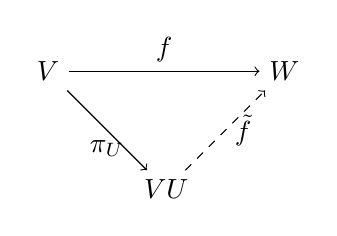
\begin{tikzpicture}
		\node (V) at (0,0) {$V$};
		\node (W) at (3,0) {$W$};
		\node (R) at (1.5,-1.5) {\qraum{$V$}{$U$}};
		\draw[->, above] (V) to node {$f$} (W);
		\draw[->, below] (V)  to node {$\pi_U$} (R);
		\draw[->, right, dashed] (R)  to node {$\tilde f$} (W);
		\end{tikzpicture}
	\end{center}
	Diese erfüllt $\Ker(\tilde f)=$\qraum{$\Ker(f)$}{U}$=\{x+U\mid x\in \Ker(f)\}\subseteq$\qraum{$V$}{$U$}.
\end{theorem}
\begin{proof}
	Ist $f=\tilde f\circ \pi_U$, so gilt $\tilde f(x+U)=\tilde f(\pi_U)=f(x)\; (*)$, somit ist $\tilde f$ dann eindeutig bestimmt. Umgekehrt 
	wird durch $(*)$ eine wohldefinierte Abbildung $\tilde f$ erklärt: Sind $x,x'\in V$ mit $x+U=x'+U$, so ist $x-x'\in U\subseteq \Ker(f)$ und 
	deshalb $f(x)=f(x')$. \\
	\begin{itemize}
		\item Linearität: Für $x,y\in V$ und $\lambda\in K$ ist $\tilde f(\lambda(x+U)+\mu(y+U))=\tilde f(\lambda\pi_U(x)+\mu\pi_U(y))=\lambda\tilde f
		(x+U)+\mu\tilde f(y+U)$.
		\item Kern: $\tilde f(x+U)=0\iff f(x)=0 \iff x\in \Ker(f)$.
	\end{itemize}
\end{proof}

\begin{conclusion}
	\proplbl{3_7_10}
	Für $f\in \Hom_K(V,W)$ ist $\Image(f)\cong $\qraum{$V$}{$\Ker(f)$}. Insbesondere gilt: Ist $f$ ein Epimorphismus, so 
	ist $W\cong $\qraum{$V$}{$\Ker(f)$}.
\end{conclusion}
\begin{proof}
	Betrachte $\tilde f:$\qraum{$V$}{$\Ker(f)$}$\to W$. Nach \propref{3_7_9} ist $\Ker(\tilde f)=$\qraum{$\Ker(f)$}{$\Ker(f)$}$=\{\Ker(f)\}$, 
	also $\tilde f$ injektiv. Nach Definition ist $\tilde f($\qraum{$V$}{$\Ker(f)$}$)=f(V)=\Image(f)$. Somit ist $\tilde f:$\qraum{$V$}
	{$\Ker(f)$}$\to \Image(f)$ ein Isomorphismus.
\end{proof}

\begin{proposition}
	\proplbl{3_7_11}
	Seien $U,U'$ Untervektorraum von $V$. Genau dann ist $V=U\oplus U'$, wenn $\pi_U|_{U'}: U'\to$\qraum{$V$}{$U$} ein Isomorphismus 
	ist.
\end{proposition}
\begin{proof}
	\begin{itemize}
		\item $\pi_U|_{U'}$ injektiv $\iff \Ker(\pi_U|_{U'})=\{0\}\iff \Ker(\pi_U)\cap U'=\{0\}\iff U\cap U'=\{0\}$
		\item $\pi_U|_{U'}$ surjektiv $\iff \forall x\in V \exists u'\in U: \pi_U(u')=\pi_U(x)\iff u'-x\in \Ker(\pi_U)=U\iff x=u+u'\iff V=U+U'$
	\end{itemize}
\end{proof}

\begin{conclusion}
	\proplbl{3_7_12}
	Ist $\dim_K(V)<\infty$, so ist $\dim_K($\qraum{$V$}{$U$}$)=\dim_K(V)-\dim_K(U)$.
\end{conclusion}
\begin{proof}
	Nach \propref{2_4_10} existiert ein lineares Komplement $U'$ zu $U$ in $V$ (d.h. $V=U\oplus U'$) und $\dim_K(U')=\dim_K(V)-\dim_K(U)$. Es gilt \qraum{$V$}
	{$U$}=$U'$.
\end{proof}

\begin{conclusion}
	\proplbl{3_7_13}
	Ist $\dim_K(V)<\infty$ und $f\in \Hom_K(V,W)$, so ist $\dim_K(V)=\dim_K(\Ker(f))+\dim_K(\Image(f))$.
\end{conclusion}
\begin{proof}
	\propref{3_7_11} und \propref{3_7_12}
\end{proof}

\begin{conclusion}
	\proplbl{3_7_14}
	Ist $\dim_K(V)<\infty$ und $f\in \End_K(V)$, so sind äquivalent:
	\begin{itemize}
		\item $f\in \Aut_K(V)$
		\item $f$ ist injektiv
		\item $f$ ist surjektiv
	\end{itemize}
\end{conclusion}
\begin{proof}
	\begin{itemize}
		\item $2\iff \dim_K(\Ker(f))=0$
		\item $3\iff \dim_K(\Image(f))=\dim_K(V)$
	\end{itemize}
\end{proof}

\begin{remark}
	Analog zu dem Quotientenräumen kann man definieren:
	\begin{itemize}
		\item Quotientengruppen \qraum{$G$}{$N$}, wobei $N$ Normalteiler von $G$ ist
		\item Quotientenringe \qraum{$R$}{$I$}, wobei $I$ ein Ideal von $R$ ist (z.B. \qraum{$\mathbb Z$}{$n\mathbb Z$})
	\end{itemize}
	Diese werden in der Vorlesung \textit{Algebra und Zahlentheorie} behandelt.
\end{remark}
\section{Rang}

Seien $V,W$ zwei endlichdimensionale $K$-Vektorräume und $f\in \Hom_K(V,W)$.

\begin{definition}[Rang]
	Der \begriff{Rang} von $f$ ist $\rk(f)=\dim_K(\Image(f))$.
\end{definition}

\begin{definition}[Rang einer Matrix]
	Der Rang einer \begriff[Rang!]{Matrix} $A\in \Mat_{m\times n}(K)$ ist $\rk(A)=\rk(f_A)$, wobei $f_A:K^n\to K^m$ 
	die durch $A$ beschriebene lineare Abbildung ist.
\end{definition}
\section{Lineare Gleichungssysteme}

Sei $A\in \Mat_{m\times n}(K)$ und $b\in K^m$.

\begin{definition}[Lineares Gleichungssystem]
	Unter einem \begriff{Linearen Gleichungssystem} verstehen wir eine Gleichung der Form $Ax=b$. 
	Diese heißt \begriff{homogen}, wenn $b=0$, sonst \begriff{inhomogen} und $L(A,b)=\{x\in K^n\mid Ax=b\}$ ist sein \begriff{Lösungsraum}.
\end{definition}

\begin{mathematica}[Lineare Gleichungssysteme]
	Für das Lösen von Linearen Gleichungssystemen gibt es in WolframAlpha bzw. Mathematica verschiedene Verfahren:
	\begin{itemize}
		\item \texttt{Solve[]}:
		\begin{align}
			\texttt{Solve[a == 2 b \&\& b == 5 \&\& c + a == b, \{a, b, c\}]}\notag
		\end{align}
		\item \texttt{LinearSolve[]}: Braucht 2 Argumente: Zum einen die Koeffizientenmatrix $A$ und den Ergebnisvektor $b$. Rückgabe ist dann der Variablenvektor $x$.
		\begin{align}
			\texttt{LinearSolve[\{\{1, 1\}, \{0, 1\}\}, \{6, 10\}]}\notag
		\end{align}
	\end{itemize}
\end{mathematica}

\begin{remark}
	Ist $A=(a_{ij})$, $b=(b_1,...,b_m)^t$, so schreibt man das Lineare Gleichungssystem $Ax=b$ auch
	\begin{align}
	\begin{vmatrix}
		a_{11}x_1 + \dots + a_{1n}x_n & = & b_1\\
		\vdots & \vdots & \vdots\\
		a_{m1}x_1 + \dots + a_{mn}x_n & = & b_m\\
	\end{vmatrix}\notag
	\end{align}
\end{remark}

\begin{remark}
	Das homogene System $Ax=0$ hat als Lösungsraum den Untervektorraum $L(A,0)=\Ker(f_A)$ der Dimension $\dim_K(L(A,0))=n-\rk(A)$. Das 
	inhomogene System hat entweder $L(A,b)=\emptyset$ oder der Lösungsraum ist der affine Unterraum $L(A,b)=f^{-1}(b)=x_0+L(A,0)$, wobei 
	$x_0\in L(A,b)$ beliebig. Man erhält so alle Lösungen des inhomogenen Systems, wenn man eine Lösung und die Lösungen des homogenen 
	Systems kennt.
\end{remark}

\begin{definition}[Zeilenstufenform]
	Die Matrix $A=(a_{ij})$ hat \begriff{Zeilenstufenform}, wenn es ganze Zahlen $0\le r \le m$ und $1\le 
	k_1<...<k_r\le n$ gibt mit:
	\begin{itemize}
		\item für $1\le i \le r$ und $1\le j < k_i$ ist $a_{ij}=0$
		\item für $1\le i \le r$ ist $a_{ik_{i}}\neq 0$ (sogenannte \begriff{Pivotelemente})
		\item für $r<i\le m$ und $1\le j\le n$ ist $a_{ij}=0$
	\end{itemize}
	\begin{align}
		\begin{pmatrix}
		0 & \dots & 0 & a_{1k_{1}} & * & \dots & \dots & *\\
		0 & \dots & \dots & 0 & a_{2k_{2}} & * & \dots & *\\
		\vdots & \vdots & \vdots & \vdots & \vdots & \vdots & \vdots & \vdots\\
		0 & \dots & \dots & \dots & \dots & \dots & \dots & a_{rk_{r}}\\
		0 & \dots & \dots & \dots & \dots & \dots & \dots & 0\\
		\vdots & \; & \; & \; & \; & \; & \; & \vdots\\
		0 & \dots & \dots & \dots & \dots & \dots & \dots & 0\\
		\end{pmatrix}\notag
	\end{align}
\end{definition}

\begin{lemma}
	Sei $A$ in Zeilenstufenform. Dann ist $\rk(A)=r$.
\end{lemma}
\begin{proof}
	Wegen $\rk(A)=\rk(A^t)=\dim_K(\ZR)$ genügt es zu zeigen, dass die ersten $r$ Zeilen $a_1,...,a_r$ linear unabhängig sind. Ist $\sum
	_{i=1}^r \lambda a_i=0$, so ist insbesondere $0=\sum_{i=1}^r \lambda_i a_{ik_{i}}=\lambda_1 a_{1k_{1}}$, also $\lambda_1
	=0$, und dann immer so weiter.
\end{proof}

\begin{proposition}
	\proplbl{3_9_6}
	Sei $A$ in Zeilenstufenform.
	\begin{itemize}
		\item Ist $b_i\neq 0$ für ein $r<i\le m$, so ist $L(A,b)=\emptyset$.
		\item Ist $b_i=0$ für alle $r<i\le m$, so erhält man alle $x\in L(A,b)$, indem man erst $x_j\in K$ für $j\in \{1,..,n\}
		\backslash \{k_1,...,k_r\}$ beliebig wählt und dann für $i=r,r-1,...,1$ rekursiv $x_{k_{i}}=a_{1k_{i}}^{-1}\cdot (b_i-\sum
		_{j=k_i+1}^n a_{ij}\cdot x_j)\quad (*)$ setzt.
	\end{itemize}
\end{proposition}
\begin{proof}
	\begin{itemize}
		\item Klar.
		\item Sicher erhält man auf diese Weise Lösungen $x\in L(A,b)$. Umgekehrt muss jede solche Lösung $(*)$ erfüllen, man erhält auf 
		diese Weise also alle.
	\end{itemize}
\end{proof}

\begin{definition}[Elementarmatrizen]
	Für $i,j\in \{1,...,m\}$, $\lambda \in K^{\times}$ und $\mu\in K$ definieren wir 
	$m\times m$-Matrizen, die sogenannten \begriff{Elementarmatrizen}:
	\begin{itemize}
		\item $S_i(\lambda):=1_m + (\lambda-1)E_{ii}$
		\item $Q_{ij}(\mu):= 1_m + \mu E_{ij}$
		\item $P_{ij}:= 1_m + E_{ij} + E_{ji} - E_{ii} - E_{jj}$
	\end{itemize}
\end{definition}

\begin{remark}
	Multiplikation einer dieser Matrizen von links an die Matrix $A$ hat folgende Wirkung:
	\begin{itemize}
		\item $S_i(\lambda)\cdot A$: Multiplikation der $i$-ten Zeile mit $\lambda$
		\item $Q_{ij}(\mu)\cdot A$: Addition des $\mu$-fachen der $j$-ten Zeile zur $i$-ten Zeile
		\item $P_{ij}$: Vertauschung von $i$-ter und $j$-ter Zeile
	\end{itemize}
	Man spricht dann von sogenannten elementaren Zeilenumformungen der Matrix $A$ von Typ I, II oder III.
\end{remark}

\begin{lemma}
	Es sind $S_i(\lambda),Q_{ij}(\mu),P_{ij}\in \GL_m(K)$. Dann ist $S_i(\lambda)^{-1}=S_i(\lambda^{-1}), Q_{ij}(\mu)
	^{-1}=Q_{ij}(-\mu),P_{ij}^{-1}=P_{ij}$. Insbesondere gilt: Ist $E$ eine der Elementarmatrizen, so ist $\ZR(EA)=\ZR(A)$ und $L(EA,0)=
	L(A,0)$. Weiterhin ist $\rk(EA)=\rk(A)$.
\end{lemma}
\begin{proof}
	Inverse nachprüfen. Da $E\in \GL_m(K)$ sind $f_E,f_{E^t}\in Aut_K(K^m)$, also $\ZR(EA)=\SR((EA)^t)=\Image(f_{A^tE^t})=\Image(f_{A^t}\circ
	f_{E^t})=\Image(f_{A^t})=\ZR(A)$ und $L(EA,0)=\Ker(f_{EA})=\Ker(f_E\circ f_A)=\Ker(f_A)=L(A,0)$.
\end{proof}

\begin{remark}
	Anders gesagt: Elementare Zeilenumformungen verändern den Lösungsraum eines homogenen linearen Gleichungssystems 
	nicht.
\end{remark}

\begin{theorem}[Eliminierungsverfahren nach \person{Gauß}]
	\proplbl{3_9_11}
	Zu jeder Matrix $A\in \Mat_{m\times n}(K)$ gibt es $l\in \mathbb N_0$ und 
	Elementarmatrizen $E_1,...,E_l$ vom Typ II und III für die $E_l\cdot ... \cdot E_1\cdot A$ in Zeilenstufenform ist. 
\end{theorem}
\begin{proof}
	Seien $a_1,...,a_n$ die Spalten von $A$. \\
	Ist $A=0$ so ist nichts zu tun. \\
	Sei nun $A\neq 0$ und sei $k_1$ minimal mit $a_{k_1}\neq 0$. Es gibt also ein $i$ mit $a_{ik_1}\neq 0$. Durch Vertauschen der ersten 
	und der $i$-ten Zeile erreichen wir, dass $a_{1k_1}=0$, d.h. wir multiplizieren $A$ mit $E_1=P_{1i}$. Nun addieren wir für $i=2,..,m$ 
	ein geeignetes Vielfaches der ersten Zeile zur $i$-ten Zeile, um $a_{ik_1}=0$, d.h. wir multiplizieren $A$ mit $E_i=Q_{i1}(\mu_i)$ für 
	$\mu_i=\frac{a_{ik_1}}{a_{1k_1}}$. Nach diesen Umformungen haben wir eine Matrix der Form:
	\begin{align}\begin{pmatrix}
		0 & \dots & 0 & a_{1k_1} & * & \dots & *\\
		0 & \dots & \dots & 0 & \textcolor{red}{*} & \textcolor{red}{\dots} & \textcolor{red}{*}\\
		\vdots & \vdots & \vdots & \vdots & \textcolor{red}{\vdots} & \textcolor{red}{\vdots} & \textcolor{red}{\vdots}\\
		0 & \dots & \dots & 0 & \textcolor{red}{*} & \textcolor{red}{\dots} & \textcolor{red}{*}\\
		\end{pmatrix}\notag\end{align}
	und können nun mit dem \textcolor{red}{Rest der Matrix $A=:A'$} von vorne beginnen. Die nun folgenden Zeilenumformungen werden die 
	erste Zeile und die ersten $k_1$ Spalten nicht mehr ändern, und weil $A'$ weniger Zeilen und Spalten als $A$ hat, bricht das Verfahren 
	nach endlich vielen Schritten ab.
\end{proof}

\begin{mathematica}[\person{Gauss}-Verfahren]
	Auch für das \person{Gauss}-Verfahren hat Mathematica bzw. WolframAlpha eine Funktion. Sie gibt die Matrix nach Ausführung des \person{Gauss}-Algorithmus zurück.
	\begin{align}
		\texttt{RowReduce[\{\{1, 4\}, \{2, 5\}\}]}\notag
	\end{align}
\end{mathematica}

\begin{conclusion}
	Zu jeder Matrix $A$ gibt es eine invertierbare Matrix $S\in \GL_n(K)$ für die $SA$ in Zeilenstufenform ist.
\end{conclusion}
\begin{proof}
	folgt direkt aus \propref{3_9_11} mit $S=E_l\cdot ... \cdot E_1$
\end{proof}

\begin{remark}
	Der Beweis für das Eliminierungsverfahren (\propref{3_9_11}) liefert ein Verfahren, die Elementarmatrizen $E_1,...,E_l$ zu finden. 
	Damit erhält man ein Verfahren ein lineares Gleichungssystem zu lösen. Setzt man $S=E_l\cdot ... \cdot E_1$, $A'=SA$ und $b'=Sb$, so 
	ist $L(A,b)=L(A',b')$: $Ax=b\Rightarrow SAx=Sb$ bzw. $A'x=b' \Rightarrow S^{-1}A'x=S^{-1}b'$. \\
	Das Gleichungssystem kann dann mit \propref{3_9_6} gelöst werden. Praktisch führt man die elementaren Zeilenumformungen an $A$ parallel dazu auch an $b$ 
	durch.
\end{remark}

\begin{remark}
	Es gibt von diesem Verfahren verschiedene Varianten und weitere Anwendungen: So kann man z.B. die Invertierbarkeit 
	einer Matrix $A\in \Mat_n(K)$ prüfen und ggf. das Inverse bestimmen: Ist $E_l\cdot ... \cdot E_1\cdot A$ in Zeilenstufenform, so ist $A$ 
	genau dann invertierbar, wenn alle Zeilen von Null verschieden sind. Ist dies der Fall, so ist $r=n$ und $k_i=i$ für alle $i$, 
	und man findet weitere Elementarmatrizen $E_{l+1},...,E_s$ vom Typ I und II, für die $E_s\cdot ... \cdot E_1\cdot A=1_n$. Dann ist 
	$S'=E_s\cdot ... \cdot E_1\cdot A=A^{-1}$ (vgl. \propref{3_8_11}). Praktisch erhält man $A^{-1}$, indem man die Zeilenumformungen an $A$ parallel dazu 
	auch an $1_n$ ausführt.
\end{remark}

\begin{conclusion}
	Jedes $A\in \GL_m(K)$ ist ein Produkt von Elementarmatrizen.
\end{conclusion}
\begin{proof}
	$A^{-1}=S'=E_s\cdot ... \cdot E_1 \Rightarrow A=(E_s\cdot ... \cdot E_1)^{-1}=E_1^{-1}\cdot ... \cdot E_s^{-1}$
\end{proof}

\chapter{Determinanten}
\section{Das Vorzeichen einer Permutation}

In diesem Kapitel sei $K$ ein Körper und $R$ ein kommutativer Ring mit Einselement.

\begin{definition}[Fehlstand, Vorzeichen]
	Sei $\sigma\in S_n$.
	\begin{itemize}
		\item Ein \begriff{Fehlstand} von $\sigma$ ist ein Paar $(i,j)$ mit $1\le i<j\le n$ und $\sigma(i)>\sigma(j)$.
		\item Das \begriff{Vorzeichen} (oder \begriff{Signum}) von $\sigma$ ist $\sgn(\sigma)=(-1)^{f(\sigma)}\in \{-1,1\}$, wobei $f(\sigma)$ die 
		Anzahl der Fehlstände von $\sigma$ ist.
		\item Man nennt $\sigma$ \begriff[Vorzeichen!]{gerade}, wenn $\sgn(\sigma)=1$, sonst \begriff[Vorzeichen!]{ungerade}.
	\end{itemize}
\end{definition}
\section{Determinante einer Matrix}

\begin{remark}
	Wir werden nun auch Matrizen mit Koeffizienten in Ring $R$ anstatt $K$ betrachten. Mit der gewohnten Addition und 
	Multiplikation bilden die $n\times n$-Matrizen einen Ring $\Mat_n(R)$, und wir definieren wieder $\GL_n(R)=\Mat_n(R)^{\times}$.
\end{remark}

\begin{remark}
	Seien $a_1,...,a_n\in R^m$ Spaltenvektoren, so bezeichnen wir mit $A=(a_1,...,a_n)\in \Mat_{m\times n}(R)$ die 
	Matrix mit den Spalten $a_1,...,a_n$. sind $\widetilde{a_1},...,\widetilde{a_m}\in R^n$ Zeilenvektoren, so bezeichnen wir mit $\tilde A=(
	\widetilde{a_1},...,\widetilde{a_m})\in \Mat_{m\times n}(R)$ die Matrix mit den Zeilen $\widetilde{a_1},...,\widetilde{a_m}$.
\end{remark}

\begin{remark}
	\proplbl{4_2_3}
	Wir hatten bereits definiert: $\det(A)=ad-bc$ (\propref{3_1_13}) mit 
	\begin{align}
		A=\begin{pmatrix}a&b\\c&d\end{pmatrix}\in \Mat_2(K)\notag
	\end{align} und hatten 
	festgestellt: $\det(A)\neq 0 \iff A\in \GL_2(K)$. Interpretation im $K=\mathbb R$:\\
	\begin{center}
		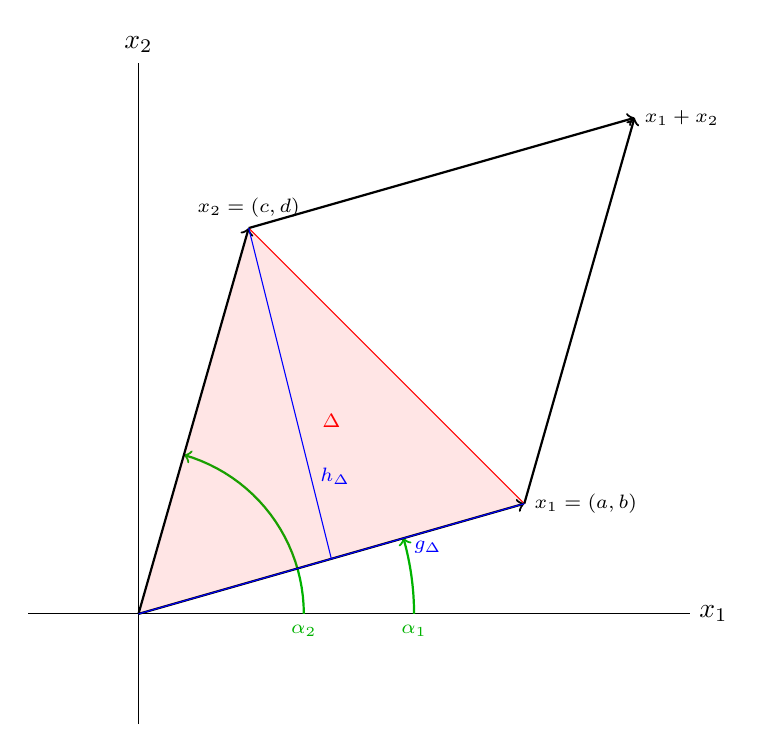
\begin{tikzpicture}[scale=0.7]
		\draw[thin] (-2,0) -- (10,0) node[right] {$x_1$}; 
		\draw[thin] (0,-2) -- (0,10) node[above] {$x_2$};
		%circles
		\draw [->,green!70!black,thick,domain=0:16] plot ({5*cos(\x)}, {5*sin(\x)});
		\draw [green!70!black] (5,-0.3) node {\scriptsize $\alpha_1$};
		\draw [->,green!70!black,thick,domain=0:74] plot ({3*cos(\x)}, {3*sin(\x)});
		\draw [green!70!black] (3,-0.3) node {\scriptsize $\alpha_2$};
		% triangle
		\fill[line width=1pt, color=red,fill=red, opacity=0.1] (0,0) -- (2,7) -- (7,2) -- cycle ;
		\draw[red] (2,7) -- (7,2);
		\draw[red] (3.5,3.5) node {\scriptsize $\Delta$};
		% Paralello
		\draw[->, thick] (0,0) -- (7,2) node[right] {\scriptsize $x_1=(a,b)$};
		\draw[->, thick] (0,0) -- (2,7) node[above] {\scriptsize$x_2=(c,d)$};
		\draw[->, thick] (7,2) -- (9,9) node[right] {\scriptsize$x_1 + x_2$};
		\draw[->, thick] (2,7) -- (9,9);
		\draw[blue] (0,0) -- (7,2) node[near end, below] {\scriptsize $g_{\Delta}$};
		\draw[blue] (3.5,1) -- (2,7) node[near start, right] {\scriptsize$h_{\Delta}$};
		\end{tikzpicture}
	\end{center}
	Parallelogramm hat die Fläche $|\det A|$. Polarkoordinaten: $x_i=\lambda_i(\cos a_i, \sin a_i)$. Ohne Einschränkung: $0\le a_1 \le a_2
	\le \pi$
	\begin{align}
	F_{P} &= 2\cdot F_{\Delta} = 2\cdot \frac 1 2 \cdot g_{\Delta} \cdot h_{\Delta} \notag \\
	g_{\Delta} &= \lambda_1 \notag \\
	h_{\Delta} &= \lambda_2 \cdot \sin(a_2-a_1) \notag \\
	F_{P} &= \lambda_1\lambda_2(\cos a_1 \sin a_2 - \sin a_1 \cos a_2) = \det(\begin{pmatrix}\lambda_1 \cos a_1 & 
	\lambda_1 \sin a_1 \\ \lambda_2 \cos a_2 & \lambda_2 \sin a_2 \end{pmatrix}) \notag \\
	&= \det A \notag
	\end{align}
	Insbesondere erfüllt $\det$ die folgenden Eigenschaften: 
	\begin{itemize}
		\item Für $\lambda\in R$ ist $\det(\lambda x_1,x_2)=\det(x_1,\lambda x_2)=\lambda\cdot \det(x_1,x_2)$
		\item Für $x_i=x'_i+x''_i$ ist $\det(x_1,x_2)=\det(x'_1,x_2) + \det(x''_1,x_2)$
		\item Ist $x_1=x_2$, so ist $\det A=0$
		\item $\det(\mathbbm{1}_2)=1$
	\end{itemize}
\end{remark}

\begin{definition}[Determinantenabbildung]
	Eine Abbildung $\delta:\Mat_n(R)\to R$ heißt \begriff{Determinantenabbildung}, wenn gilt:
	\begin{itemize}
		\item (D1): $\delta$ ist linear in jeder Zeile: sind $a_1,...,a_n$ die Zeilen von $A$ und ist $i\in \{1,...,n\}$ und $a_i=\lambda'a'_i + 
		\lambda''a''_i$ mit $\lambda',\lambda''\in R$ und den Zeilenvektoren $a'_i,a''_i$, so ist $\delta(A)=\lambda'\cdot \delta(a_1,...,
		a'_i,...,a_n) + \lambda''\cdot \det(a_1,...,a''_i,...,a_n)$.
		\item (D2): $\delta$ ist alternierend: sind $a_1,...,a_n$ die Zeilen von $A$ und $i,j\in \{1,...,n\}$, $i\neq j$ mit $a_i=a_j$, so ist 
		$\delta(A)=0$.
		\item (D3): $\delta$ ist normiert: $\delta(\mathbbm{1}_n)=1$.
	\end{itemize}
\end{definition}

\begin{mathematica}[Determinante]
	Die Determinante einer Matrix lässt sich in Mathematica bzw. WolframAlpha wie folgt berechnen:
	\begin{align}
		\texttt{Det[\{\{1, 4\}, \{2, 5\}\}]}\notag
	\end{align}
\end{mathematica}

\begin{example}
	\proplbl{4_2_5}
	Sei $\delta:\Mat_n(K)\to K$ eine Determinantenabbildung. Ist $A\in \Mat_n(K)$ nicht invertierbar, so sind die Zeilen 
	$a_1,...,a_n$ von $A$ linear abhängig, es gibt also ein $i$ mit $a_i=\sum_{j\neq i} \lambda_j\cdot a_j$. Es folgt $\delta(A)=
	\delta(a_1,...,a_n)=\sum_{j\neq i} \lambda_j\cdot \delta(a_1,...,a_j,...,a_n)$ mit $a_i=a_j$ mit D2: $\sum_{j\neq i} 
	\lambda_j\cdot 0=0=\delta(A)$.
\end{example}

\begin{lemma}
	\proplbl{4_2_6}
	Erfüllt $\delta:\Mat_n(R) \to R$ die Axiome D1 und D2, so gilt für jedes $\sigma\in S_n$ und die Zeilenvektoren 
	$a_1,...,a_n$: 
	\begin{align}
		\delta(a_{\sigma(1)},...,a_{\sigma(n)})=\sgn(\sigma)\cdot \delta(a_1,...,a_n)\notag
	\end{align}
\end{lemma}
\begin{proof}
	 $\sigma$ ist ein Produkt von Transpositionen. Es genügt also die Behauptung für $\sigma=\tau_{ij}$ mit $1\le i<j\le n$ zu zeigen (\propref{4_1_7}). \\
	 \begin{align}
	 	0&=\delta(a_1,...,a_i+a_j,...,a_j+a_i,....,a_n) \notag \\
	 	&=\delta(a_1,...,a_i,...,a_j,...,a_n)+\delta(a_1,...,a_i,...,a_i,...,a_n)+\delta(a_1,...,a_j,
	 	...,a_j,...,a_n)+\delta{a_1,...,a_j,...,a_i,...,a_n} \notag \\
	 	&=\delta(a_1,...,a_n)+\delta(a_{\sigma(1)},...,a_{\sigma(n)}) \notag \\
	 	&=0 \notag
	 \end{align}
	 Mit $\sgn(\sigma)=
	 \sgn(\tau_{ij})=-1$ folgt die Behauptung.
\end{proof}

\begin{lemma}
	\proplbl{4_2_7}
	Erfüllt $\delta:\Mat_n(R)\to R$ die Axiome D1 und D2, so gilt für $A=(a_{ij})\in \Mat_n(R)$: 
	\begin{align}
		\delta(A)=\delta(\mathbbm{1}_n)
		\cdot \sum_{\sigma\in S_n} \left( \prod_{i=1}^n a_{i,\sigma(i)} \right)\notag
	\end{align}
\end{lemma}
\begin{proof}
	Schreibe $a_i=(a_{j_1},...,a_{in})=\sum_{j=1}^n a_{ij}\cdot e_j$. Wiederholtes Anwenden von D1 gibt 
	\begin{align}
		\delta(A)&=\delta(a_1,...,a_n) \notag \\
		&=\sum_{j_1=1}^n a_{1j_1}\cdot \delta(e_{j_1},a_2,...,a_n) \notag \\
		&=\sum_{j_1=1}^n ... \sum_{j_n=1}^n \delta(e_{j_1},...,e_{j_n})\cdot \prod_{i=1}^n a_{ij_i} \notag
	\end{align}
	Wegen D2 ist $\delta(e_{j_1},...,e_{j_n})=0$ falls $j_i=j_{i'}$ für ein $i\neq i'$. 
	Andernfalls ist $\sigma(i)=j_i$ einer Permutation von $\{1,...,n\}$ und 
	\begin{align}
		\delta(e_{j_1},...,e_{j_n})&=\delta(e_{\sigma(1)},...,e_{\sigma(n)}) \notag \\
		&=\sgn(\sigma)\cdot \delta(e_1,...,e_n) \notag \\
		&=\sgn(\sigma)\cdot \delta(\mathbbm{1}_n) \notag
	\end{align}
	nach \propref{4_2_6}.
\end{proof}

\begin{theorem}
	\proplbl{4_2_8}
	Es gibt genau eine Determinantenabbildung $\delta:\Mat_n(R)\to R$ und diese ist gegeben durch die 
	Leibnitzformel 
	\begin{align}
		\det(a_{ij})=\sum_{\sigma\in S_n} \sgn(\sigma)\cdot \prod_{i=1}^n a_{i,\sigma(i)} = \sum_{\sigma
			\in A_n}\prod_{i=1}^n a_{i,\sigma(i)} - \sum_{\sigma\in S_n\backslash A_n}\prod_{i=1}^n a_{i,\sigma(i)}\notag
	\end{align}
\end{theorem}
\begin{proof}
	Eindeutigkeit der Abbildung folgt wegen D3 aus \propref{4_2_7}. Bleibt nur noch zu zeigen, dass $\det$ auch die Axiome D1 bis D3 erfüllt. \\
	D1: klar \\
	D3: klar \\
	D2: Seien $\mu\neq v$ mit $a_{\mu}=a_v$. Mit $\tau=\tau_{\mu v}$ ist $S_n\backslash A_n = A_n\tau$, somit 
	\begin{align}
		\det(a_{ij})&=
		\sum_{\sigma\in A_n} \prod_{i=1}^n a_{i,\sigma(i)}-\sum_{\sigma\in A_n\tau} \prod_{i=1}^n a_{i,\sigma\tau(i)} \notag \\
		&=
		\sum_{\sigma\in A_n} \left( \prod_{i=1}^n a_{i,\sigma(i)} - \prod_{i=1}^n a_{i,\sigma\tau(i)} \right) \notag
	\end{align}
	nach \propref{4_1_10}. Da $a_{ij}=a_{\tau(i),j}$ 
	für alle $i,j$ ist 
	\begin{align}
		\prod_{i=1}^n a_{i,\sigma(i)}&=\prod_{i=1}^n a_{\tau(i),\sigma\tau(i)} \notag \\
		&=\prod_{i=1}^n a_{i,\sigma\tau(i)} \notag
	\end{align}
	für jedes $\sigma\in S_n$, woraus $\det(a_{ij})=0$ folgt.
\end{proof}

\begin{example}
	\proplbl{4_2_9}
	\begin{itemize}
		\item $n=2$, $S_2=\{\id, \tau_{12}\}$, 
		\begin{align}
			A=\begin{pmatrix}a_{11} & a_{12} \\ a_{21}  & a_{22}\end{pmatrix}\notag
		\end{align}
		$\det(A)=\sum_{\sigma\in
			S_2} a_{1,\sigma(1)}\cdot a_{2,\sigma(2)}=a_{11}\cdot a_{22} - a_{12}\cdot a_{21}$
		\item $n=3$, $S_3=\{id,\tau_{12}, \tau_{23}, \tau_{13}, \text{2 zyklische Vertauschungen}\}$, $A_3=\{\id, \text{2 zyklische 
			Vertauschungen}\}$, $S_3\backslash A_3=\{\tau_{12},\tau_{23},\tau_{13}\}$ und
		\begin{align}
			A=\begin{pmatrix}
			a_{11} & a_{12} & a_{13} \\
			a_{21} & a_{22} & a_{23} \\
			a_{31} & a_{32} & a_{33} \\
			\end{pmatrix}\notag
		\end{align}
		ergibt sich: $\det(A)=\sum_{\sigma\in A_3} a_{1,\sigma(1)}\cdot a_{2,\sigma(2)}\cdot a_{3,\sigma(3)} - \sum_
		{\sigma\in S_3\backslash A_3} a_{1,\sigma(1)}\cdot a_{2,\sigma(2)}\cdot a_{3,\sigma(3)}= a_{11}a_{22}a_{33} + a_{12}a_{23}
		a_{31} + a_{13}a_{21}a_{32} - a_{12}a_{21}a_{33} - a_{13}a_{22}a_{31} - a_{11}a_{23}a_{32}$
		\item Ist $A=(a_{ij})$ eine obere Dreiecksmatrix, so ist $\det(A)=\prod_{i=1}^n a_{ii}$
		\item Für $i\neq j$, $\lambda\in K^{\times}$, $\mu\in K$ ist $\det(S_i(\lambda))=\lambda$, $\det(Q_{ij}(\mu))=1$, $\det(P_{ij})=-1$
		\item Ist $A$ eine \begriff{Blockmatrix} der Gestalt 
		\begin{align}
			\begin{pmatrix}A_1 & C \\ 0 & A_2\end{pmatrix}\notag
		\end{align} mit quadratischen Matrizen $A_1,
		A_2,C$, so ist $\det(A)=\det(A_1)\cdot \det(A_2)$
	\end{itemize}
\end{example}

\begin{conclusion}
	Für $A\in \Mat_n(R)$ ist $\det(A)=\det(A^t)$. Insbesondere erfüllt $\det$ die Axiome D1 und D2 auch für Spalten 
	anstatt Zeilen.
\end{conclusion}
\begin{proof}
	Mit $\rho=\sigma^{-1}$ gilt $\sgn(\rho)=\sgn(\sigma)$ nach \propref{4_1_8} und somit 
	\begin{align}
		\det(A)&=\sum_{\sigma\in S_n} \sgn(\sigma) \cdot \prod_
		{i=1}^n a_{i,\sigma(i)} \notag \\
		&=\sum_{\rho\in S_n} \sgn(\rho)\cdot \prod_{i=1}^n a_{\rho(i),i} \notag \\
		&=\det(A^t) \notag
	\end{align}
	nach \propref{4_2_8}.
\end{proof}

\begin{theorem}[Determinantenmultiplikationssatz]
	\proplbl{4_2_11}
	Für $A,B\in \Mat_n(R)$ ist 
	\begin{align}
		\det(AB)=\det(A)\cdot \det(B)\notag
	\end{align}
\end{theorem}
\begin{proof}
	Fixiere $A$ und betrachte die Abbildung $\delta: \Mat_n(R)\to R$ mit $B\mapsto \det(AB^{-1})$. Diese Abbildung erfüllt die Axiome 
	D1 und D2. sind $b_1,...,b_n$ die Zeilen von $B$, so hat $AB^{-1}$ die Spalten $Ab_1^t,...,Ab_n^t$, es werden die Eigenschaften 
	von $\det$ auf $\delta$ übertragen. \\
	$\Rightarrow \det(AB)=\delta(B^t)=\delta(\mathbbm{1}_n)\cdot \det(B^t)=\det(A)\cdot \det(B)$.
\end{proof}

\begin{conclusion}
	\proplbl{4_2_12}
	Die Abbildung $\det:\Mat_n(R)\to R$ schränkt sich zu einem Gruppenhomomorphismus $\GL_n(R)\to 
	R^{\times}$ ein. Ist $R=K$ ein Körper, so ist $A\in \Mat_n(K)$ also genau dann invertierbar, wenn $\det(A)\neq 0$ und in 
	diesem Fall ist $\det(A^{-1})=\det(A)^{-1}$.
\end{conclusion}
\begin{proof}
	Aus $AA^{-1}=\mathbbm{1}_n$ folgt $\det(A^{-1})*\det(A)=\det(\mathbbm{1}_n)=1$, insbesondere $\det(A)\in R^{\times}$. Der zweite Teil folgt wegen 
	$K^{\times}=K\backslash \{0\}$ (\propref{4_2_5}).
\end{proof}

\begin{conclusion}
	Die Matrizen mit Determinante 1 bilden einen Normalteiler $\SL_n(K)=\{A\in \GL_n \mid \det(A)=1\}$ der 
	allgemeinen linearen Gruppe, die sogenannte \begriff{spezielle lineare Gruppe}.
\end{conclusion}

\begin{conclusion}
	\proplbl{4_2_14}
	Elementare Zeilenumformungen vom Typ II ändern die Determinante nicht, elementare Zeilenumformungen vom 
	Typ III ändern nur das Vorzeichen der Determinante.
\end{conclusion}
\begin{proof}
	$\det(Q_{ij}(\mu)A)=\det(Q_{ij}(\mu)) \cdot \det(A)= 1\cdot \det(A) = \det(A)$ (\propref{4_2_9}), Rest analog.
\end{proof}

\begin{remark}
	Aus \propref{4_2_14} und \propref{4_2_9} erhält man eine praktische Methode zur Berechnung der Determinante. Man bringt die Matrix mit dem \person{Gauss}-Algorithmus \propref{3_9_11} auf Zeilenstufenform, bildet das Produkt über die Diagonale und multipliziert mit -1, falls am eine ungerade Anzahl von Zeilenvertauschungen vorgenommen hat.
\end{remark}
\section{Minoren}

Seien $m,n\in \mathbb N$.

\begin{definition}[adjungierte Matrix]
	Sei $A=(a_{ij})\in \Mat_n(R)$. Für $i,j\in \{1,...,n\}$ definieren wir die $n\times n$-Matrix: \\
	\begin{align}
		A_{ij}=\begin{pmatrix}
		a_{11} & ... & a_{1,j-1} & 0 & a_{1,j+1} & ... & a_{1n} \\
		\vdots & \ddots & \vdots & \vdots & \vdots & \ddots & \vdots \\
		a_{i-1,1} & ... & a_{i-1,j.1} & 0 & a_{i-1,j+1} & ... & a_{i-1,n} \\
		0 & ... & 0 & 1 & 0 & ... & 0 \\
		a_{i+1,1} & ... & a_{i+1,j.1} & 0 & a_{i+1,j+1} & ... & a_{i+1,n} \\
		\vdots & \ddots & \vdots & \vdots & \vdots & \ddots & \vdots \\
		a_{n1} & ... & a_{n,j-1} & 0 & a_{n,j+1} & ... & a_{nn} \\
		\end{pmatrix}\notag
	\end{align}
	die durch Ersetzen der $i$-ten Zeile und der $j$-ten Spalte durch $e_j$ aus $A$ hervorgeht, sowie die $(n-1)\times(n-1)$-
	Matrix: \\
	\begin{align}
		A'_{ij}=\begin{pmatrix}
		a_{11} & ... & a_{1,j-1} & a_{1,j+1} & ... & a_{1n} \\
		\vdots & \ddots & \vdots & \vdots & \ddots & \vdots \\
		a_{i-1,1} & ... & a_{i-1,j.1} & a_{i-1,j+1} & ... & a_{i-1,n} \\
		a_{i+1,1} & ... & a_{i+1,j.1} & a_{i+1,j+1} & ... & a_{i+1,n} \\
		\vdots & \ddots & \vdots & \vdots & \ddots & \vdots \\
		a_{n1} & ... & a_{n,j-1} & a_{n,j+1} & ... & a_{nn} \\
		\end{pmatrix}\notag
	\end{align}
	die durch Streichen der $i$-ten Zeile und der $j$-ten Spalten entsteht. Weiterhin definieren wir die zu $A$ \begriff{adjungierte Matrix} 
	als $A^\#=(a_{ij}^\#)\in \Mat_n(R)$, wobei $a_{ij}^\#=\det(A_{ji})$.
\end{definition}

\begin{lemma}
	Sei $A\in \Mat_n(R)$ mit Spalten $a_1,...,a_n$. Für $i,j\in \{1,..,n\}$ gilt:
	\begin{itemize}
		\item $\det(A_{ij})=(-1)^{i+j}\cdot \det(A'_{ij})$
		\item $\det(A_{ij})=\det(a_1,...,a_{j-1},e_i,a_{j+1},...,a_n)$
	\end{itemize}
\end{lemma}
\begin{proof}
	\begin{itemize}
		\item Durch geeignete Permutation der ersten $i$ Zeilen und der ersten $j$ Zeilen erhält man 
		\begin{align}
			\det(A_{ij})&=(-1)^{(i-1)+
				(j-1)} \cdot \det(\begin{pmatrix}1&0&...&0 \\ 0 & \; & \; & \; \\ \vdots & \; & A'_{ij} & \; \\ 0 & \; & \; & \; \\ \end{pmatrix})\notag \\
			&=(-1)^{i+j}\cdot \det(\mathbbm{1}_n)\cdot \det(A'_{ij})\notag
		\end{align}
		\item Man erhält $A_{ij}$ aus $(a_1,...,e_i,...,a_n)$ durch elementare Spaltenumformungen vom Typ II.
	\end{itemize}
\end{proof}

\begin{proposition}
	\proplbl{4_3_3}
	Für $A\in \Mat_n(R)$ ist 
	\begin{align}
		A^\#\cdot A=A\cdot A^\#=\det(A)\cdot \mathbbm{1}_n
	\end{align}
\end{proposition}
\begin{proof}
	$(A^\#A)_{ij}=\sum_{k=1}^n a^\#_{ik}\cdot a_{kj}=\sum_{k=1}^n a_{kj}\cdot \det(A_{kj})=\sum_{k=1}^n a_{kj}\cdot 
	\det(a_1,...,a_{i-1},a_j,a_{i+1},...,a_n)=\det(a_1,...,a_{i-1},\sum_{k=1}^n a_{kj}e_k,a_{i+1},...,a_n) = \det(a_1,...,a_{i-1},a_j,
	a_{i+1},...,a_n)=\delta_{ij}\cdot \det(A)=(\det(A)\cdot \mathbbm{1}_n)_{ij}$. Analog bestimmt man die Koeffizienten von $AA^\#$, wobei man 
	$\det(A_{jk})=\det(A_{jk}^t)=\det((A^t)_{kj})$ benutzt.
\end{proof}

\begin{conclusion}
	Es ist $\GL_n(R)=\{A\in \Mat_n(R) \mid \det(A)\in R^{\times}\}$ und für $A\in \GL_n(R)$ ist $A^{-1}=
	\frac{1}{\det(A)}\cdot A^\#$.
\end{conclusion}
\begin{proof}
	\propref{4_3_3} und \propref{4_2_12}
\end{proof}

\begin{proposition}[\person{Laplace}'scher Entwicklungssatz]
	Sei $A=(a_{ij})\in \Mat_n(R)$. Für jedes $i,j\in \{1,..,n\}$ gilt die 
	Formel für die Entwicklung nach der $i$-ten Zeile: \\
	\begin{align}
		\det(A)=\sum_{j=1}^n (-1)^{i+j}\cdot a_{ij}\cdot \det(A'_{ij})\notag
	\end{align}
	Gleiches gilt auch für Spalten.
\end{proposition}
\begin{proof}
	$\det(A)=(AA^\#)_{ij}=\sum_{j=1}^n a_{ij}\cdot a^\#_{ij} = \sum_{j=1}^n a_{ij}\cdot \det(A_{ij})=\sum_
	{j=1}^n a_{ij}\cdot (-1)^{i+j}\cdot \det(A'_{ij})$. Analog auch für Spalten.
\end{proof}

\begin{proposition}[\person{Cramer}'sche Regel]
	Sei $A\in \GL_n(R)$ mit Spalten $a_1,...,a_n$ und sei $b\in R^n$. Weiter sei 
	$x=(x_1,...,x_n)^t\in R^n$ die eindeutige Lösung des Linearen Gleichungssystems $Ax=b$. Dann ist für $i=1,...,n$ 
	\begin{align}
		x_i=\frac{\det(a_1,...,a_{i-1},b,a_{i+1},...,a_n)}{\det(A)}\notag
	\end{align}
\end{proposition}
\begin{proof}
	$x_i=(A^{-1}b)_i=\sum_{j=1}^n (A^{-1})_{ij}\cdot b_j=\frac{1}{\det(A)}\cdot \sum_{j=1}^n a^\#_{ij}\cdot b_j = 
	\frac{1}{\det(A)}\cdot \sum_{j=1}^n b_j\cdot \det(a_1,...,a_{i-1},e_i,a_{i+1},...,a_n)=\frac{1}{\det(A)}\cdot \det(a_1,...,
	a_{i-1},b_j,a_{i+1},...,a_n)$.
\end{proof}

\begin{definition}[Minor]
	Sei $A=(a_{ij})\in \Mat_{m\times n}(R)$ und $1\le r \le m$, $1\le s \le n$. Eine $r\times s$-
	Teilmatrix von $A$ ist eine Matrix der Form $(a_{i\mu,jv})_{\mu,v}\in \Mat_{r\times s}(R)$ mit $1\le i_1<...<i_r\le m$ 
	und $1\le j_1<...<j_s\le n$. Ist $A'$ eine $r\times r$-Teilmatrix von $A$, so bezeichnet man $\det(A')$ als einen 
	$r$-\begriff{Minor} von $A$.
\end{definition}

\begin{example}
	Ist $A\in \Mat_n(R)$ und $i,j\in \{1,...,n\}$, so ist $A'_{ij}$ eine Teilmatrix und $\det(A'_{ij})=(-1)^{i+j}
	\cdot a^\#_{ji}$ ein $(n-1)$-Minor von $A$.
\end{example}

\begin{proposition}
	Sei $A\in \Mat_n(R)$ und $r\in \mathbb N$. Genau dann ist $\rk(A)\ge r$, wenn es eine $r\times r$-
	Teilmatrix $A'$ von $A$ mit $\det(A^{\prime})\neq 0$ gibt.
\end{proposition}
\begin{proof}
	\begin{itemize}
		\item Hinrichtung: Ist $\rk(A)\ge r$, so hat $A$ $r$ linear unabhängige Spalten $a_1,...,a_r$. Die Matrix $\tilde A=(a_1,...,a_r)$ 
		hat den Rang $r$ und deshalb $r$ linear unabhängige Zeilen $\widetilde{a_1},...,\widetilde{a_r}$. Die $r\times r$-Matrix $A$ hat 
		dann Rang $r$, ist also invertierbar, und $\det(A)\neq 0$.
		\item Rückrichtung: Ist $A'$ eine $r\times r$-Teilmatrix von $A$ mit $\det(A')\neq 0$, so ist $\rk(A)\ge \rk(A')=r$.
	\end{itemize}
\end{proof}

\begin{conclusion}
	Sei $A\in \Mat_{m\times n}(K)$. Der Rang von $A$ ist das größte $r\in \mathbb N$, für das 
	$A$ einen von Null verschiedenen $r$-Minor hat.
\end{conclusion}
\section{Determinante und Spur von Endomorphismen}

Sei $n\in \mathbb N$ und $V$ ein $K$-Vektorraum mit $\dim_K(V)=m$.

\begin{proposition}
	\proplbl{4_4_1}
	Sei $f\in \Hom_K(V,W)$, $A'$ eine Basis von $V$ und $A=M_{A'}(f)$. Sei weiter $B\in \Mat_n(K)$. Genau 
	dann gibt es eine Basis $B'$ von $V$ mit $B=M_{B'}(f)$, wenn es $S\in \GL_n(K)$ mit $B=SAS^{-1}$ gibt.
\end{proposition}
\begin{proof}
	Ist $B'$ eine Basis von $V$ mit $B=M_{B'}(f)$, so ist $B=SAS^{-1}$ mit $S=T^{A'}_{B'}$. Sei umgekehrt $B=SAS^{-1}$ mit 
	$S\in \GL_n(K)$. Es gibt eine Basis $B'$ von $V$ mit $T^{A'}_{B'}=S$, also $M_{B'}(f)=T^{A'}_{B'}\cdot M_{A'}(f)\cdot (
	T^{A'}_{B'})^{-1}=SAS^{-1}=B$: Mit $B'=(\Phi_{A'}(f_s^{-1}(e_1)),...,\Phi_{A'}(f_s^{-1}(e_n)))$ ist $\Phi_{A'}\circ f_s^{-1}=
	\id_V\circ \Phi_{B'}$, also $T^{A'}_{B'}=M_{A'}^{A'}(\id_V)=S^{-1}$. Folglich ist $T^{A'}_{B'}=(T_{A'}^{B'})^{-1}=(S^{-1})^{-1}
	=S$ nach \propref{3_6_2}.
\end{proof}

\begin{definition}[Ähnlichkeit]
	Zwei Matrizen $A,B\in \Mat_n(R)$ heißen \begriff{ähnlich}, wenn (in Zeichen $A\sim B$) es 
	$S\in \GL_n(R)$ mit $B=SAS^{-1}$ gibt.
\end{definition}

\begin{proposition}
	Ähnlichkeit von Matrizen ist eine Äquivalenzrelation auf $\Mat_n(R)$.
\end{proposition}
\begin{proof}
	\begin{itemize}
		\item Reflexivität: $A=\mathbbm{1}_n\cdot A \cdot (\mathbbm{1}_n)^{-1}$
		\item Symmetrie: $B=SAS^{-1}\Rightarrow A=S^{-1}BS=S^{-1}B(S^{-1})^{-1}$
		\item Transitivität: $B=SAS^{-1}$, $C=TBT^{-1}\Rightarrow C=TSAS^{-1}T^{-1}=(TS)A(ST)^{-1}$
	\end{itemize}
\end{proof}

\begin{proposition}
	\proplbl{4_4_4}
	Seien $A,B\in \Mat_n(R)$. Ist $A\sim B$, so ist
	\begin{align}
		\det(A)=\det(B)\notag
	\end{align}
\end{proposition}
\begin{proof}
	$B=SAS^{-1}$, $S\in \GL_n(R)$, $\det(B)=\det(S)\cdot \det(A)\cdot \det(S)^{-1}=\det(A)$ nach \propref{4_2_11} und \propref{4_2_12}
\end{proof}

\begin{definition}[Determinante eines Endomorphismus]
	Die \begriff[Endomorphismus!]{Determinante} eines Endomorphismus $f\in \End_K(V)$ ist 
	\begin{align}
		\det(f)=\det(M_B(f))\notag
	\end{align}
	wobei $B$ eine Basis von $V$ ist. (Diese ist wohldefiniert nach \propref{4_4_1} und \propref{4_4_4})
\end{definition}

\begin{proposition}
	\proplbl{4_4_6}
	Für $f,g\in \End_K(V)$ gilt:
	\begin{itemize}
		\item $\det(\id_V)=1$
		\item $\det(f\circ g)=\det(f)\cdot \det(g)$
		\item Genau dann ist $\det(f)\neq 0$, wenn $f\in \Aut_K(V)$. In diesem Fall ist $\det(f^{-1})=\det(f)^{-1}$
	\end{itemize}
\end{proposition}
\begin{proof}
	\begin{itemize}
		\item klar
		\item folgt aus \propref{3_6_6} und \propref{4_2_11}
		\item folgt aus \propref{3_6_5} und \propref{4_2_12}
	\end{itemize}
\end{proof}

\begin{definition}[Spur einer Matrix]
	Die \begriff[Matrix!]{Spur} einer Matrix $A=(a_{ij})\in \Mat_n(R)$ ist 
	\begin{align}
		\tr(A)=\sum_{i=1}^n a_{ii}\notag
	\end{align}
\end{definition}

\begin{mathematica}[Spur einer Matrix]
	Auch für die Spur einer Matrix hat Mathematica bzw. WolframAlpha eine Funktion:
	\begin{align}
		\texttt{Tr[\{\{1, 2, 3\}, \{4, 5, 6\}, \{7, 8, 9\}\}]}\notag
	\end{align}
\end{mathematica}

\begin{lemma}
	\proplbl{4_4_8}
	Seien $A,B\in \Mat_n(R)$
	\begin{itemize}
		\item $\tr: \Mat_n(R)\to R$ ist $R$-linear
		\item $\tr(A^t)=\tr(A)$
		\item $\tr(AB)=\tr(BA)$
	\end{itemize}
\end{lemma}
\begin{proof}
	in den Übungen bereits behandelt
\end{proof}

\begin{proposition}
	\proplbl{4_4_9}
	Seien $A,B\in \Mat_n(R)$. Ist $A\sim B$, so ist $\tr(A)=\tr(B)$.
\end{proposition}
\begin{proof}
	$B=SAS^{-1}$, $S\in \GL_n(R)\Rightarrow \tr(B)=\tr(SAS^{-1})\overset{\propref{4_4_8}}{=}\tr(AS^{-1}S)=\tr(A)$
\end{proof}

\begin{definition}[Spur eines Endomorphismus]
	Die \begriff[Endomorphismus!]{Spur} eines Endomorphismus $f\in \End_K(V)$ ist
	\begin{align}
		\tr(f)=\tr(M_B(f))\notag
	\end{align} 
	wobei $B$ eine Basis von $V$ ist (Diese ist wohldefiniert nach \propref{4_4_1} und \propref{4_4_9})
\end{definition}

\begin{remark}
	Im Fall $K=\mathbb R$ kann man wie in \propref{4_2_3} den Absolutbetrag der Determinante eines $f\in \End_K(K^n)$ 
	geometrisch interpretieren, nämlich als das Volumen von $f(Q)$, wobei $Q=[0,1]^n$ der Einheitsquader ist, und somit 
	als Volumenänderung durch $f$. Auch das Vorzeichen von $\det(f)$ hat eine Bedeutung: Es gibt an, ob $f$ 
	orientierungserhaltend ist. Für erste Interpretationen der Spur siehe A100.
\end{remark}

\part*{Anhang}
\addcontentsline{toc}{part}{Anhang}
\appendix

\chapter{Listen}
\section{Liste der Theoreme}
\theoremlisttype{allname}
\listtheorems{theorem}

\pagebreak
\section{Liste der benannten Sätze}
\theoremlisttype{optname}
\listtheorems{proposition, lemma}

\pagebreak
\section{Liste der Mathematica/WolframAlpha-Befehle}
\smiley{} für faule Mathematiker \smiley{} \\
\theoremlisttype{allname}
\listtheorems{mathematica}

%\printglossary[type=\acronymtype]

\printindex

\end{document}
